\thispagestyle{toancuabinone}
\pagestyle{toancuabi}
\everymath{\color{toancuabi}}
\blfootnote{$^1$\color{toancuabi}Trường PT Hermann Gmeiner Vinh, Nghệ An.}
\graphicspath{{../toancuabi/pic2/}}
\begingroup
\AddToShipoutPicture*{\put(0,616){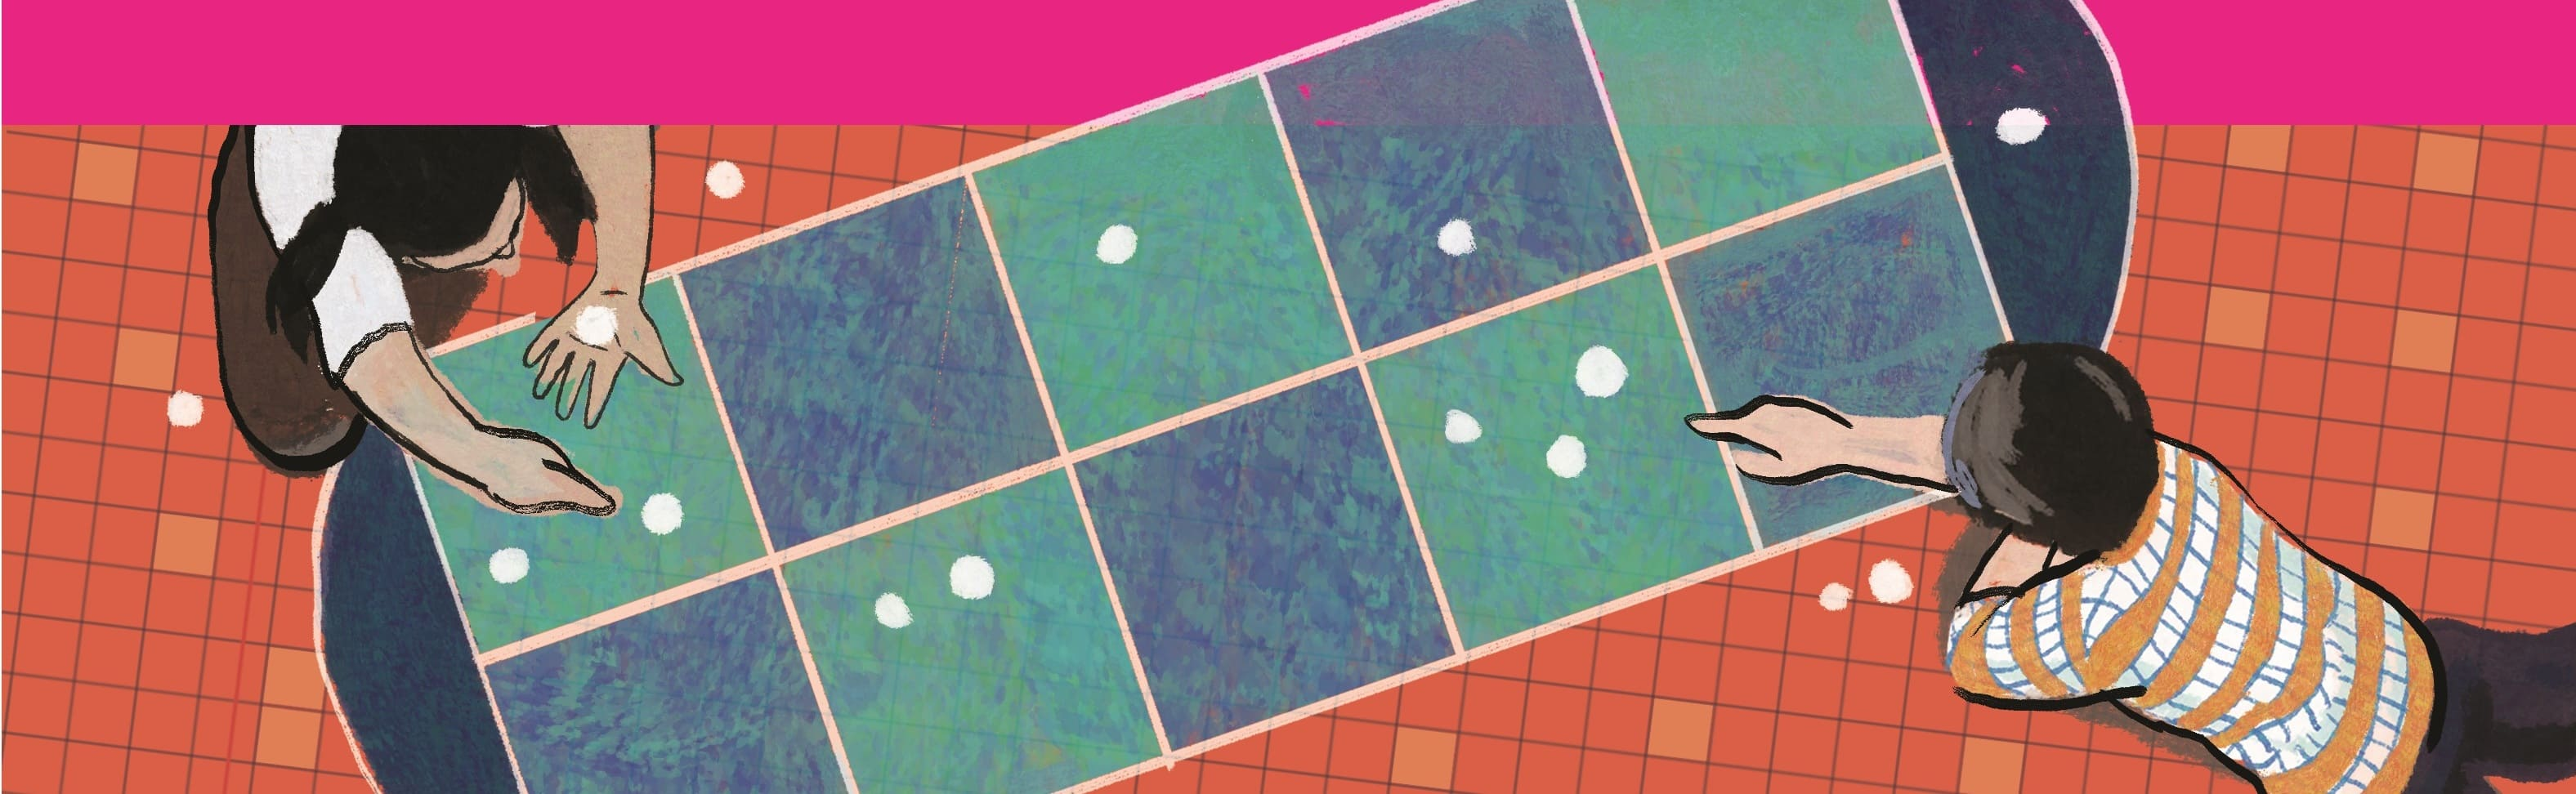
\includegraphics[width=19.3cm]{../bannertoancuabi}}}  
\AddToShipoutPicture*{\put(110,555){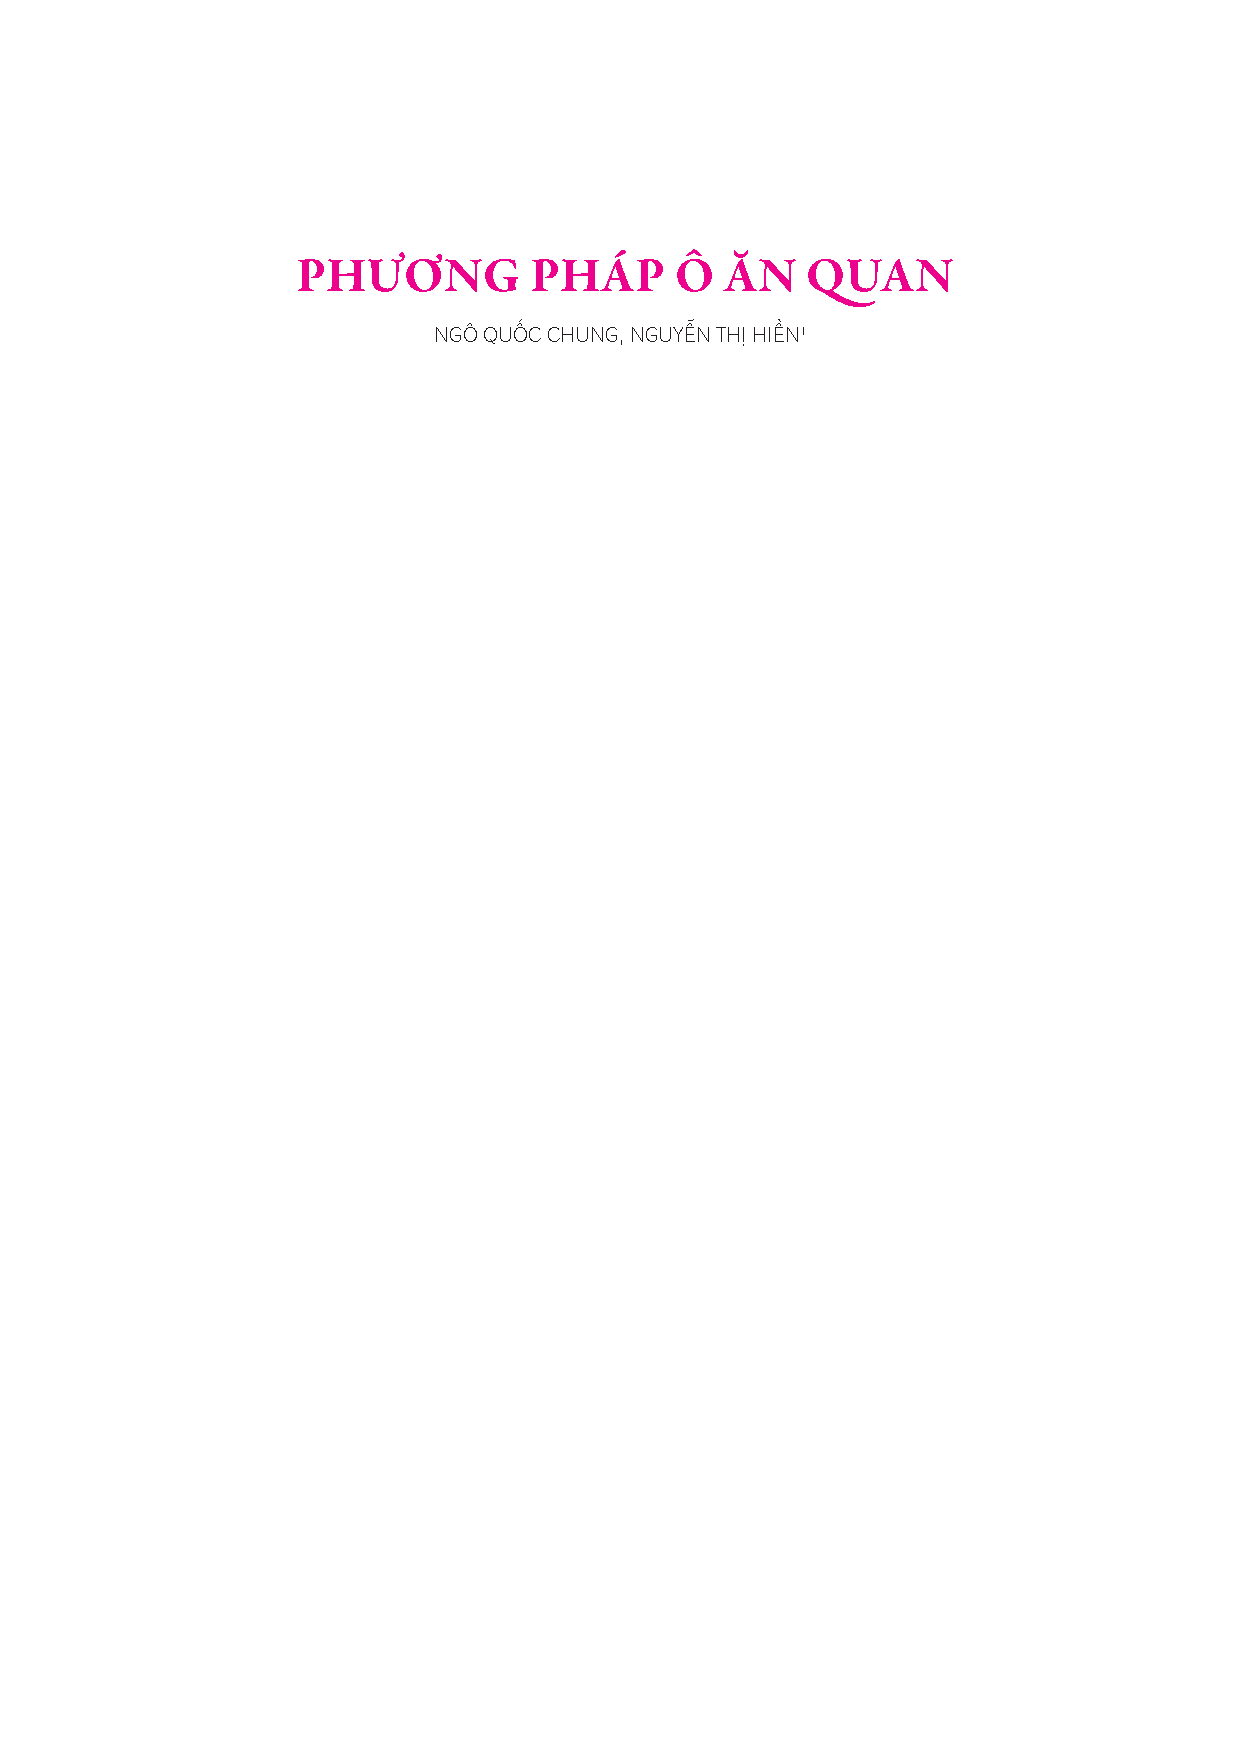
\includegraphics[scale=1]{../tieude1111.pdf}}}  
\centering
\endgroup
\vspace*{160pt} 

	\textit{\textbf{\color{toancuabi}LTS.} Trong số này, tạp chí Pi giới thiệu đến bạn đọc một bài viết đạt giải trong kỳ thi Bài giảng và bài viết Toán học, mang tên Hoàng Tuỵ, năm $2022$. Bài viết về chủ đề giảng dạy Toán theo chương trình Toán học $2018$ -- Chương trình Giáo dục Phổ thông mới.}
\begin{multicols}{2}
	\textbf{\color{toancuabi}I.	Đặt vấn đề}
	\vskip 0.1cm
	Trong quá trình tìm các Bài toán thực tế, và xem trò chơi dân gian ``Ô ăn quan" chúng tôi phát hiện ra có sự tương đồng rất lớn giữa bài toán tập hợp hữu hạn với tập hợp các viên sỏi trong trò chơi ``Ô ăn quan". Từ đó chúng tôi nghĩ đến câu hỏi có thể sử dụng phương pháp ô ăn quan để giải các bài Toán tập hợp đếm được, hữu hạn hay không? Áp dụng cho một số Bài toán ban đầu chúng tôi thấy cách giải là rất đẹp và dễ hiểu. Chúng tôi đặt tên cho cách giải đó là ``phương pháp ô ăn quan"
	\vskip 0.1cm
	Với ý muốn là sẽ tạo một cách giải hết sức trực quan chúng tôi quyết định nghiên cứu sâu hơn về các Bài toán tập hợp được phát biểu dưới dạng các bài Toán cổ, ngoài ra chúng ta có thể giải quyết được một số bài ở mức độ phức tạp hơn, khi chứa nhiều biến trong một bài toán.
	\vskip 0.1cm
	Môn toán trong chương trình phổ thông ở cấp Tiểu học giúp học sinh có những kiến thức cơ bản và sơ giản ban đầu về số học, hình học, các yếu tố đại lượng và hình thành các kĩ năng toán học góp phần xây dựng phương pháp học tập, làm việc có kế hoạch, chủ động, sáng tạo giúp các em học tập tốt các môn học khác trong nhà trường và chuẩn bị cho các bậc học tiếp theo. Trong bài viết này, chúng tôi sẽ giải một lớp các Bài toán đó bằng phương pháp ``Ô ăn quan",các ví dụ đưa ra là những bài toán rất quen thuộc ở Tiểu học và cả một số bài tập đề cập ở trên chương trình Toán THPT.
	\vskip 0.1cm
	Với ý tưởng như trên, bài viết sẽ trình bày những kết quả đạt được đạt được trong quá trình chuyển tải phương pháp ``Ô ăn quan" vào giải các bài Toán tập hợp của chương trình Toán Phổ thông mới.
	\vskip 0.1cm
	\textbf{\color{toancuabi}II.	Giải các Bài toán tập hợp bằng phương pháp ``Ô ăn quan"}
	\vskip 0.1cm
	Các bài toán cổ dưới đây thường có nhiều phương pháp giải mà mỗi bậc học có thể được trang bị một cách khác nhau. Tuy nhiên đây là các bài toán có tính logic cao nên học sinh phải có năng lực Toán học khá mới dùng được các phương pháp như vẽ biểu đồ, đặt ẩn giải hệ phương trình, hoặc dùng biểu đồ Venn. Trong phương pháp ô ăn quan, chúng tôi sử dụng những mô tả rất thực tế qua việc dùng những viên sỏi; ô trống và rải sỏi dẫn đến học sinh không cần đòi hỏi quá nhiều kiến thức về Toán vẫn có thể lĩnh hội được.
	\vskip 0.1cm
	\textbf{\color{toancuabi}Bài toán $\pmb{1}$: Gà và chó}
	\begin{center}
		``Vừa gà vừa chó,\\
		Bó lại cho tròn,\\
		$36$ con, $100$ chân chẵn."
	\end{center}
	Hỏi có bao nhiêu con gà, bao nhiêu con chó?
	\vskip 0.1cm
	\textit{Lời giải.}
	Theo bài ta có: tổng số con gà và con chó có tất cả $36$ con và $100$ chân.
	\vskip 0.1cm
	Bây giờ ta vẽ $36$ ô và dùng $100$ viên sỏi. Trong $36$ ô, mỗi ô ta rải vào $2$ viên sỏi hết $72$ viên sỏi, còn lại $28$ viên sỏi. Rải tiếp $28$ viên sỏi còn lại vào các ô, mỗi ô thêm $2$ viên sỏi. Khi đó, có $14$ ô chứa $4$ viên sỏi và $22$ ô chứa $2$ viên sỏi. Vậy ta có $14$ con chó và $22$ con gà.
	\begin{figure}[H]
		\vspace*{-5pt}
		\centering
		\captionsetup{labelformat= empty, justification=centering}
		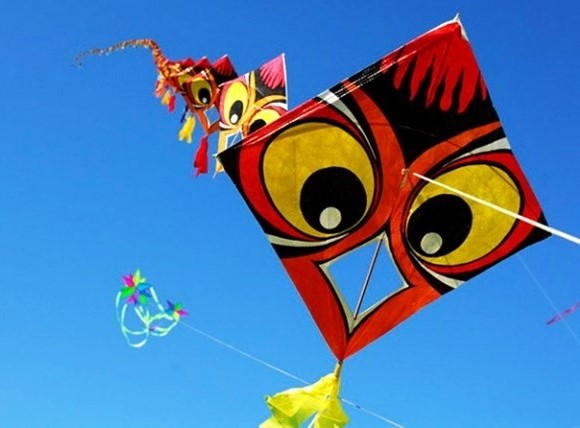
\includegraphics[width= 1\linewidth]{1}
		\vspace*{-15pt}
	\end{figure}
	\textbf{\color{toancuabi}Bài toán $\pmb2$: Thuyền to -- Thuyền nhỏ}
	\begin{center}
		``Thuyền to chở được $6$ người,\\
		Thuyền nhỏ chở được $4$ người là đông.\\
		Một đoàn trai gái sang sông,\\
		$10$ thuyền to nhỏ giữa dòng đang trôi.\\
		Toàn đoàn có cả $100$ người, Trên bờ còn $48$ người đợi sang"
	\end{center}
	Hỏi có bao nhiêu thuyền to, bao nhiêu thuyền nhỏ
	\vskip 0.1cm
	\textit{Lời giải}.
	Toàn đoàn có $100$ người, trên bờ còn $48$ người đợi sang, như vậy có $52$ người đang ngồi trên $10$ thuyền.
	\vskip 0.1cm
	Theo bài ta có: Tổng số thuyền nhỏ và to là $10$ thuyền, $52$ người.
	\vskip 0.1cm
	Bây giờ ta vẽ $10$ ô và dùng $52$ viên sỏi. Trong $10$ ô mỗi ô ta rải vào $4$ viên sỏi hết $40$ viên sỏi, còn lại $12$ viên sỏi. Bỏ tiếp $12$ viên sỏi còn lại vào các ô, mỗi ô thêm $2$ viên. Khi đó, có $6$ ô chứa $6$ viên sỏi và $4$ ô chứa $4$ viên sỏi. Hay có $6$ thuyền to và $4$ thuyền nhỏ.
	\begin{figure}[H]
		\vspace*{5pt}
		\centering
		\captionsetup{labelformat= empty, justification=centering}
		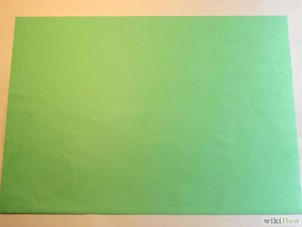
\includegraphics[width= 1\linewidth]{2}
		\vspace*{-15pt}
	\end{figure}
	\textit{Nhận xét.}
	Thông qua những ví dụ trên ta thấy phương pháp ô ăn quan sử dụng những trực quan cụ thể, giúp học sinh dễ dàng thực hiện và ghi nhớ cách làm đồng thời tìm ra kết quả chính xác.
	\vskip 0.1cm
	Ví dụ trên đã yêu cầu học sinh vận dụng được sự mềm dẻo, linh hoạt trong suy nghĩ để giải quyết bài toán. Đó là một yếu tố rất cần thiết, tránh sự cứng nhắc rập khuôn theo những phương pháp đã dẫn đến những cách giải cồng kềnh hoặc bế tắc.
	\vskip 0.1cm
	\textbf{\color{toancuabi}Bài toán $\pmb3$: Bài toán lợn và gà}
	\begin{center}
		Tối qua đếm đàn lợn gà\\
		Thấy được trăm mắt còn đầu năm mươi\\
		Một trăm hai chục chân tròn\\
		Đố bạn biết có bao nhiêu gà và lợn?
	\end{center}
	\textit{Lời giải.}
	Có $50$ cái đầu nên tổng số lợn và gà là $50$ con và tổng số là $120$ chân. Bây giờ ta vẽ $50$ ô tượng trưng cho $50$ con, và lấy $120$ viên sỏi tượng trưng cho $120$ cái chân.
	\vskip 0.1cm
	Bây giờ ta sẽ rải đầy kín tất cả các ô, với mỗi ô hoặc hai viên sỏi, hoặc $4$ viên sỏi. Khi đó số ô có $4$ viên tức là có $4$ chân chính là lợn, số ô có $2$ viên tức là có $2$ chân chính là gà.
	\vskip 0.1cm
	Rõ ràng khi rải đầy các ô có hai viên mỗi ô, thì hết $100$ viên, nên thừa $20$ viên, $20$ viên còn lại rải đủ cho $10$ ô, và do đó để thêm mỗi ô $2$ viên. Vậy số ô có $4$ viên là $10$ nên số lợn là $10$ con, còn lại số ô có $2$ viên là $40$ ô vậy có $40$ gà.
	\begin{figure}[H]
		\vspace*{-5pt}
		\centering
		\captionsetup{labelformat= empty, justification=centering}
		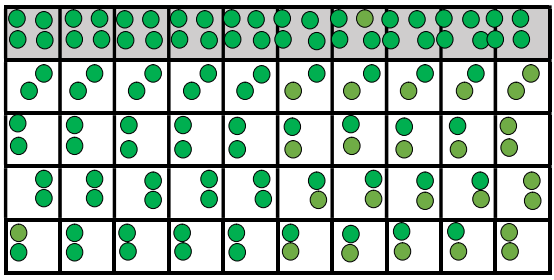
\includegraphics[width= 1\linewidth]{3}
		\vspace*{-15pt}
	\end{figure}
	\textbf{\color{toancuabi}Bài toán $\pmb4$: Bài toán ``Thương nhau cau sáu bổ ba"}
	\begin{center}
		`Thương nhau cau sáu bổ ba\\
	Ghét nhau cau sáu bổ ra làm mười.\\
	 Mỗi người một miếng trăm người,\\
	Có mười bảy quả hỏi người ghét yêu"?
	\end{center}
	Hỏi có bao nhiêu quả cau ghét và bao nhiêu quả cau yêu.
	\vskip 0.1cm
	\textit{Lời giải.}
	Ta coi $17$ quả cau là $17$ ô vuông và $100$ miếng cau chia cho $100$ người là $100$ viên sỏi. Trong $17$ ô vuông, mỗi ô vuông rải $3$ viên sỏi hết $51$ viên sỏi, còn lại $49$ viên sỏi. Rải tiếp $49$ viên còn lại vào các ô, mỗi ô thêm $7$ viên. Khi đó, có $7$ ô chứa $10$ viên sỏi và $10$ ô chứa $3$ viên sỏi. Hay có $30$ người tương ứng với $10$ quả cau bổ $3$ và $70$ người ghét ứng với $7$ quả cau bổ $10$.
	\begin{figure}[H]
		\vspace*{-5pt}
		\centering
		\captionsetup{labelformat= empty, justification=centering}
		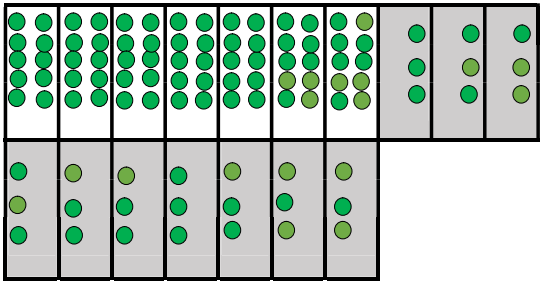
\includegraphics[width= 1\linewidth]{4}
		\vspace*{-15pt}
	\end{figure}
	\textbf{\color{toancuabi}Bài toán $\pmb6$: (Buôn cà phê)}
	\vskip 0.1cm
	Người nọ mua một số cafe tốt và một số cafe xấu trộn lại cân nặng $50$ kg, trả tất cả $7.800\$$. Biết rằng giá $1$ kg cafe tốt $180\$$, giá $1$ kg cafe xấu $120\$$. Hỏi người ấy mua mỗi hạng cafe mấy kg?
	\vskip 0.1cm
	\textit{Lời giải}.
	Ta coi mỗi ô là $1$ kg cà phê, có $50$ kg cà phê nên sẽ có $50$ ô, bây giờ ta sẽ xem mỗi viên sỏi là $60\$$, tổng cộng là $7800\$$ nên sẽ ứng với $130$ viên sỏi. Sau đó ta sẽ rải sỏi vào các ô, mà mỗi ô chỉ nhận $2$ viên $=120\$$ hoặc $3 $viên $=180\$$, số ô có $3$ viên chính là cà phê tốt, số ô chỉ có $2$ viên chính là cà phê xấu. Đầu tiên ta rải đủ $50$ ô, mỗi ô $2$ viên thì còn lại $30$ viên, ta tiểp tục rải $30$ viên còn lại mỗi ô thêm $1$ viên cho đến khi hết sỏi. Ta có hình vẽ sau.
	\begin{figure}[H]
		\vspace*{5pt}
		\centering
		\captionsetup{labelformat= empty, justification=centering}
		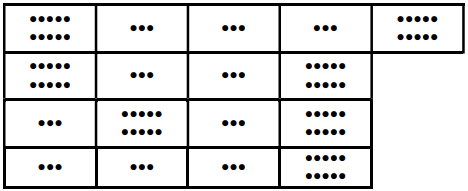
\includegraphics[width= 1\linewidth]{5}
		\vspace*{-15pt}
	\end{figure}
	Nhìn vào bảng ta thấy có $30$ ô chứa $3$ viên sỏi, vậy có $30$ kg cà phê tốt, có $20$ ô chứa hai viên sỏi nên có $20$ kg cà phê xấu.
	\vskip 0.1cm
	Bây giờ ta sẽ giải các bài Toán tập hợp có độ phức tạp cao hơn, đó là những bài toán và có từ $3$ biến trở lên. Những bài toán này nếu giải bằng các cách thông thường sẽ hết sức phức tạp và đòi hỏi rất nhiều kỹ thuật. Nhưng với phương pháp ``Ô ăn quan" ta sẽ có một lời giải rất dễ hiểu, đẹp đẽ và học sinh Tiểu học cũng có thể hiểu được.
	\vskip 0.1cm
	\textbf{\color{toancuabi}Bài toán $\pmb7$:}
	\vskip 0.1cm
	Lớp $5A$ có $35$ học sinh (HS) làm bài kiểm tra toán cuối Kỳ II. Đề bài gồm có $3$ bài toán. Giáo viên chủ nhiệm lớp báo cáo với Nhà trường rằng: Cả lớp mỗi em đều làm được ít nhất một bài, trong đó $20$ em giải được bài toán thứ nhất, $14$ HS giải được bài toán thứ hai, $10$ HS giải được bài toán thứ ba, $5$ HS giải được bài toán thứ hai và thứ ba, $2$ HS giải được bài toán thứ nhất và thứ hai, chỉ có một HS được $10$ điểm vì đã giải được cả ba bài. Học sinh nào giải được bài $3$ thì làm ít nhất thêm được một bài khác.
	Hỏi lớp học đó có bao nhiêu HS không dự kiểm tra?
	\vskip 0.1cm
	\textit{Lời giải}.
	Trước hết ta vẽ bảng gồm có $35$ ô ứng với $35$ em học sinh lớp $5A$. Ta lấy $20$ tấm thẻ ký hiệu là số $B1$ ứng với số lần giải được bài toán $1$, lấy $14$ thẻ ký hiệu là $B2$ ứng với $14$ lần giải được bài toán $2$, $10$ tấm thẻ đánh dấu là $B3$ ứng với $10$ lượt giải được bài toán $3$. Bây giờ ta sẽ rải thẻ vào các ô theo quy tắc đã cho. Đầu tiên ta rải $20$ tấm thẻ $B1$ vào $20$ ô, sau đó ta rải đến tấm thẻ $B2$ vào $2$ ô có thẻ $B1$ và thêm $12$ ô trống, hết thẻ $B2$ bây giờ ta rải thẻ $B3$, $1$ tấm thẻ vào ô đã có $2$ thẻ $B1$ và $B2$, tiếp tục rải $5$ thẻ vào các ô chỉ có thẻ $B2$, do làm được bài $3$ thì sẽ làm được hơn một bài do đó sẽ rải $4$ thẻ còn lại vào các ô chỉ có $B1$. Sau khi rải hết thẻ mà ô nào còn trống có nghĩa là học sinh đó không đi thi.
	\begin{figure}[H]
		\vspace*{-5pt}
		\centering
		\captionsetup{labelformat= empty, justification=centering}
		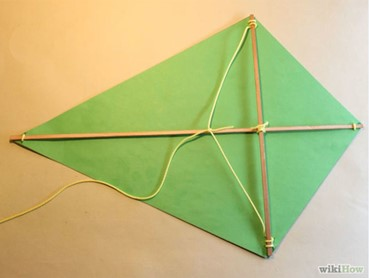
\includegraphics[width= 1\linewidth]{6}
		\vspace*{-15pt}
	\end{figure}	
	Nhìn vào bảng sau khi rải hết các thẻ theo quy tắc trên ta thấy còn lại chỉ có $3$ ô trống nên có $3$ em học sinh không tham gia thi cuối kỳ II.
	\begin{figure}[H]
		\vspace*{-5pt}
		\centering
		\captionsetup{labelformat= empty, justification=centering}
		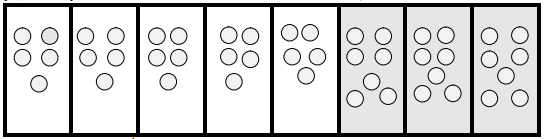
\includegraphics[width= 1\linewidth]{7}
		\vspace*{-15pt}
	\end{figure}
	\textbf{\color{toancuabi}Bài toán $\pmb8$:} 
	\vskip 0.1cm
	Trong một hội nghị có $100$ đại biểu tham dự, mỗi đại biểu nói được một hoặc hai trong ba thứ tiếng: Nga, Anh hoặc Pháp. Có $39$ đại biểu chỉ nói được tiếng Anh, $35$ đại biểu nói được tiếng Pháp, có $12$ đại biểu biết $2$ thứ tiếng trong đó $8$ đại biểu nói được cả tiếng Anh và tiếng Nga. Hỏi có bao nhiêu đại biểu chỉ nói được tiếng Nga, bao nhiêu đại biểu chỉ nói được tiếng Pháp?
	\vskip 0.1cm
	\textit{Lời giải}.
	\begin{figure}[H]
		\vspace*{-5pt}
		\centering
		\captionsetup{labelformat= empty, justification=centering}
		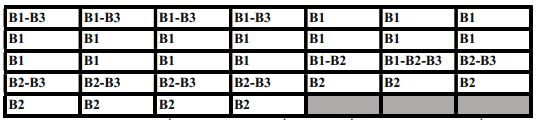
\includegraphics[width= 1\linewidth]{8}
		\vspace*{-15pt}
	\end{figure}
	Ta vẽ $100$ ô tương ứng với $100$ đại biểu. Ta sẽ làm $39$ thẻ chữ $A$ ứng với $35$ người nói được tiếng Anh, $35$ thẻ chữ $P$ ứng với $35$ người biết nói tiếng Pháp và $8$ thẻ chữ $NA$ ứng với số lượng biết nói tiếng Nga, gọi thẻ chữ $N$ là ký hiệu biết nói tiếng Nga.
	\vskip 0.1cm
	Đầu tiên, ta sẽ rải $39$ thẻ $A$ vào $39$ ô. Ta rải tiếp $35$ thẻ chữ $P$ vào các ô trống tiếp theo, tiếp tục rải tiếp $8$ thẻ $NA$ vào các ô trống còn lại. Bây giờ ta sẽ rải thẻ chữ $N$, vì mỗi đại biểu nói được ít nhất một thứ tiếng, nên những ô trống còn lại ta sẽ rải chữ $N$ vào. Do có $12$ đại biểu biết nói hai thứ tiếng mà lại có $8$ người nói Anh và Nga do đó chắc chắn có $4$ người nói tiếng Pháp thì nói được tiếng Nga (vì không thể cùng biết cả Anh và Pháp) do đó ta sẽ rải $4$ thẻ chữ $N$ vào $4$ ô có chữ $P$. Khi đó ô nào mà chỉ có một mình chữ N là chỉ nói được tiếng Nga, những ô chỉ có chữ $P$ là chỉ nói được tiếng Pháp. Nhìn vào bảng ta thấy: có $18$ ô chữ $N$ vậy có $18$ đại biểu chỉ nói được tiếng Nga. Có $31$ ô chỉ có chữ $P$ nên có $31$ đại biểu chỉ nói được tiếng Pháp
	\vskip 0.1cm
	\textbf{\color{toancuabi}Bài toán $\pmb9$.}
	\vskip 0.1cm
	$50$ bạn học sinh lớp $12A$ đều đội $1$ trong hai loại mũ: Mũ cứng hoặc mũ mềm, đi $1$ trong $2$ loại giày đen hoặc nâu, mặc $1$ trong $2$ loại áo: trắng hoặc xanh. Có $18$ bạn đội mũ mềm, $19$ bạn đi giầy đen, $11$ bạn có áo trắng. Hỏi có thể chắc chắn có ít nhất bao nhiêu bạn vừa đi giày nâu, vừa đội mũ cứng và mặc áo xanh?
	\vskip 0.1cm
	\textit{Lời giải}.
	Ta sẽ vẽ bảng gồm $50$ ô, ta kí hiệu thẻ chữ $M$, $C$ lần lượt ứng với đội mũ mềm và mũ cứng, thẻ $Đ$, $N$ lần lượt cho giày đen và giày nâu, thẻ $T$, $X$ cho mặc áo trắng và áo xanh.
	\begin{figure}[H]
		\vspace*{-5pt}
		\centering
		\captionsetup{labelformat= empty, justification=centering}
		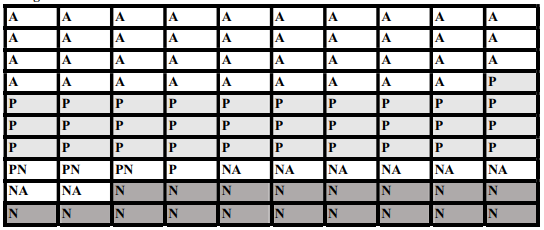
\includegraphics[width= 1\linewidth]{9}
		\vspace*{-15pt}
	\end{figure}
	Vì có $18$ bạn đội mũ mềm ta rải $18$ thẻ $M$ vào $18$ ô, các ô trống còn lại ta rải chữ $C$ cho các bạn đội mũ cứng, ta rải tiếp $19$ thẻ $D$ vào hết các bạn có thẻ chữ $C$, hết chữ $C$ ta sẽ rải sang chữ $M$, nhiều ô chữ $C$ nhất có thể. Sau đó ta rải $11$ thẻ chữ $T$ vào ô chữ $CN$, hết các ô đó ta sẽ rải sang các ô còn lại, khi hết $11$ thẻ chữ $T$ ta tiếp tục rải chữ $X$ vào tất cả các ô không chứa chữ $T$. Khi đó ô nào mà chữa $3$ chữ $CNX$ thì đó chính là học sinh đi giày Nâu, đội mũ Cứng và mặc áo Xanh.
	\vskip 0.1cm
	Nhìn vào bảng ta thấy chỉ có hai ô có $3$ chữ $CNX$ nên có ít nhất $2$ học sinh đội mũ cứng, đi giày nâu và mặc áo xanh.
	\vskip 0.1cm
	\textit{Nhận xét:} Đây là bài Toán logic khá hóc búa vì nó chứa đến $6$ yếu tố để tác động lên một học sinh, nếu dùng phương pháp suy luận thông thường chúng ta sẽ vấp phải các lý luận khá phức tạp và dễ bị nhầm lẫn. Phương pháp ``Ô ăn quan" cho ta một lời giải rất đẹp đẽ và khá ngắn gọn.
	\vskip 0.1cm
	\textbf{\color{toancuabi}IV. Bài tập đề xuất}
	\vskip 0.1cm
	\textbf{\color{toancuabi}Bài $\pmb1$:} Trong một Hội nghị có $100$ người tham dự, trong đó có $10$ người không biết tiếng Nga và tiếng Anh, có $75$ người biết tiếng Nga và $83$ người biết Tiếng Anh. Hỏi trong hội nghị có bao nhiêu người biết cả $2$ thứ tiếng Nga và Anh?
	\vskip 0.1cm
	\textbf{\color{toancuabi}Bài $\pmb2$:} Một lớp học có $16$ học sinh học giỏi môn Toán; $12$ học sinh học giỏi môn Văn; $8$ học sinh vừa học giỏi môn Toán và Văn; $19$ học sinh không học giỏi cả hai môn Toán và Văn. Hỏi lớp học có bao nhiêu học sinh?
	\vskip 0.1cm
	\textbf{\color{toancuabi}Bài $\pmb3$:} Một lớp có $45$ học sinh. Mỗi em đều đăng ký chơi ít nhất một trong hai môn: bóng đá và bóng chuyền. Có $35$ em đăng ký môn bóng đá, $15$ em đăng ký môn bóng chuyền. Hỏi có bao nhiêu em đăng ký chơi cả $2$ môn?
	\vskip 0.1cm
	\textbf{\color{toancuabi}Bài $\pmb4$:} Lớp $12A$ có $20$ học sinh thích bóng đá, $17$ học sinh thích bơi, $36$ học sinh thích bóng chuyền, $14$ học sinh thích bơi và bóng đá, $13$ học sinh thích bơi và bóng chuyền, $15$ học sinh thích bóng đá và bóng chuyền, $10$ học sinh thích cả $3$, $12$ học sinh không thích môn nào cả . Tính số học sinh của lớp $12A$?
	\vskip 0.1cm
	\textbf{\color{toancuabi}Bài $\pmb5$:} Lớp $10A$ có $40$ học sinh trong đó có $10$ bạn học sinh giỏi Toán, $15$ bạn học sinh giỏi Lý, và $22$ bạn không giỏi môn học nào trong hai môn Toán, Lý. Hỏi lớp 10A có bao nhiêu bạn học sinh vừa giỏi Toán vừa giỏi Lý?
	\vskip 0.1cm
	\textbf{\color{toancuabi}Bài $\pmb6$:} (Thi giữa kỳ $1$ -- Trường PTTH Lý Nhân Tông, Hà Nội) Lớp $10A$ có $45$ học sinh trong đó có $15$ học sinh thích chơi đá bóng, $12$ học sinh thích chơi bóng rổ, $6$ học sinh thích chơi cả $2$ môn. Số học sinh không thích chơi cả $2$ môn thể thao trên là:
	\vskip 0.1cm
	\textbf{\color{toancuabi}Bài $\pmb7$:} Lớp $10A$ có $7$ học sinh giỏi Toán, $5$ học sinh giỏi Lý, $6$ học sinh giỏi Hóa, $3$ học sinh giỏi cả Toán và Lý, $4$ học sinh giỏi cả Toán và Hóa, $2$ học sinh giỏi cả Lý và Hóa, $1$ học sinh giỏi cả $3$ môn Toán, Lý, Hóa. Số học sinh giỏi đúng hai môn học của lớp 10A là bao nhiêu.
	\vskip 0.1cm
	\textbf{\color{toancuabi}Bài $\pmb8$:} (\textit{Câu $3.48$, trang $66$, Sách BT Đại số $10$ Nâng cao})Có ba lớp học sinh $10A$, $10B$, $10C$ gồm $128$ em cùng tham gia lạo động trồng cây. Mỗi em lớp $10A$ trồng được $3$ cây bạch đàn và $4$ cây bàng. Mỗi em lớp 10B trồng được $2$ cây bạch đàn và $5$ cây bàng. Mỗi em lớp $10C$ trồng được $6$ cây bạch đàn. Cả ba lớp trồng được là $476$ cây bạch đàn và $375$ cây bàng. Hỏi mỗi lớp có bao nhiêu học sinh?
	\vskip 0.1cm
	\textbf{\color{toancuabi}Bài $\pmb9$:} (\textit{Câu $8$, trang $18$, Toán $10$ tập $1$ Sách Cánh Diều}) Một nhóm có $12$ học sinh chuẩn bị hội diễn văn nghệ. Trong danh sách đăng ký tham gia tiết mục múa và tiết mục hát của nhóm đó, có $5$ học sinh tham gia tiết mục múa và $3$ học sinh tham gia cả hai tiết mục. Hỏi có bao nhiêu học sinh trong nhóm tham gia tiết mục hát? Biết có $4$ học sinh của nhóm không tham gia tiết mục nào.
	\vskip 0.1cm
	\textbf{\color{toancuabi}Bài toán $\pmb10$:} (Câu $5$, trang $25$ sách Toán $10$ -- Chân trời sáng tạo) Trong số $35$ học sinh của lớp $10H$, có $20$ học sinh thích môn Toán, $16$ học sinh thích môn Tiếng Anh và $12$ học sinh thích cả hai môn này. Hỏi lớp $10H$:
	\vskip 0.1cm
	$a)$ Có bao nhiêu học sinh thích ít nhất một trong hai môn Toán và Tiếng Anh?
	\vskip 0.1cm
	$b)$ Có bao nhiêu học sinh không thích cả hai môn này.
	\vskip 0.1cm
	\textbf{\color{toancuabi}Tài liệu tham khảo}
	\vskip 0.1cm
	[$1$]	L. V. An, N. T. Sơn, N. T. Thiêm, N. T. H. Anh, N. Q. Chung ($2023$), Nhìn bài toán cổ theo quan điểm Tổ hợp, Kỷ yếu HTKH cấp Trường: ``Nâng cao chất lượng đào tạo ngành Sư phạm trong bối cảnh hiện nay", Trường Đại học Hà Tĩnh, (Hà Tĩnh, ngày $24/3/2023$), $179 - 186$.
	\vskip 0.1cm
	[$2$] Naum Yakolevich Vilenkin -- Dịch giả: Nguyễn Tiến Dũng, Trần Thanh Nam, Nguyễn Chí Thức, Hồ Thị Thảo Trang, \textit{Toán học qua các câu chuyện về Tập hợp}, Tủ sách SPUTNIK, NXB Thế giới, năm $2017$.
	\vskip 0.1cm
	[$3$] Trịnh Hồng Long, \textit{$670$ bài toán đố}, NXB Sống Mới, năm $1970$.
	\vskip 0.1cm
	[$4$] Người dịch: Trần Lưu Cường, Trần Lưu Thịnh, \textit{Những bài toán cổ}, NXB giáo dục, năm $1995$.
	\vskip 0.1cm
	[$4$] Trần Nam Dũng (Tổng chủ biên), Trần Đức Huyên (Chủ biên), Nguyễn Thành Anh -- Vũ Như Thư Hương -- Ngô Hoàng Long -- Phạm Hoàng Quân -- Phạm Thị Thu Thủy, \textit{Sách chân trời sáng tạo -- Toán $10$ -- Tập $1$}, NXB giáo dục Việt Nam, năm $2022$.
	\vskip 0.1cm
	[$5$]	Đỗ Đức Thái (Tổng chủ biên), Phạm Xuân Chung, Nguyễn Sơn Hà, Nguyễn Thị Phương Loan, Phạm Sỹ Nam, Phạm Minh Phương, Phạm Hoàng Quân, \textit{Sách Cánh diều -- Toán $10$ -- Tập $1$}, NXB Giáo dục, năm $2021$	
\end{multicols}
%\newpage
%\graphicspath{{../toancuabi/pic/}}
%\begingroup
%\AddToShipoutPicture*{\put(106,650){
\includegraphics[scale=1]{../tieude.pdf}}}  
%\centering
%\endgroup
%\vspace*{55pt} 
%\begin{multicols}{2}
%	Thám tử Xuân Phong đôi khi phải đột nhập vào những nơi hoang vắng, kỳ bí để tìm ra được dấu tích của những kẻ gây án. Một lần nọ, sau bao ngày cải trang để bám sát, theo dõi manh mối, thám tử biết tên trùm tội phạm đang trốn tránh trong một ngôi nhà hẻo lánh ở ngoại ô. Vừa đến trước cửa của ngôi nhà gỗ cổ kính, Xuân Phong gặp một bà lão với đôi mắt tinh anh nhìn mình với vẻ bí mật ``thám tử đó phải không, tôi nhận ngay ra ngài, dù ngài đã cải trang rất kỹ. Phải chăng thám tử đang đi tìm tên trùm? Hắn đang ngồi dưới kia, trong căn phòng cùng những người trong Hiệp hội Thương Gia, nhưng vô cùng nguy hiểm nếu ngài dùng vũ lực ở đây để bắt hắn. Tôi mách ngài nhé, ở dưới đó, có $10$ người, trong đó có lão trùm và những kẻ đồng phạm của lão. Bọn họ là những kẻ luôn nói dối, nhưng cũng có thể có cả những người lương thiện, luôn nói thật, ở ngay bên cạnh. Ngài hãy dùng trí thông minh của mình, chỉ được hỏi rất hạn chế câu hỏi để phán đoán ra những kẻ phạm tội là ai. Ngài hỏi nhiều câu hơn sẽ nguy hiểm cho cả những thương gia lương thiện có thể có mặt ở đó. Và ngài hãy hứa với bà lão này sẽ đảm bảo an toàn cho tôi và gia đình, vì tôi đã liều mình thông báo tin mật này với thám tử".
%	\vskip 0.1cm
%	Theo lời bà lão mách bảo, Xuân Phong lần theo một chiếc cầu thang cũ nát và đi xuống một căn phòng khuất dưới tầng hầm. Vừa mở cửa ra, thám tử đã thấy có $10$ người ăn mặc chỉnh tề như nhau, ngồi nghiêm trang quanh một chiếc bàn mười cạnh, mỗi người ngồi tại đỉnh của hình mười cạnh. Ánh sáng lờ mờ trong phòng đủ chiếu rõ dòng chữ ``Cuộc họp thường niên Hiệp hội Thương gia -- Khu vực Duyên Hải". Thật khó để xác định ai là kẻ nói dối trong số họ, vì vẻ ngoài họ đều giống như những thương Gia thường gặp: quyền lực, sắc sảo và oai vệ.
%	\begin{figure}[H]
	%		\centering
	%		\vspace*{-5pt}
	%		\captionsetup{labelformat= empty, justification=centering}
	%		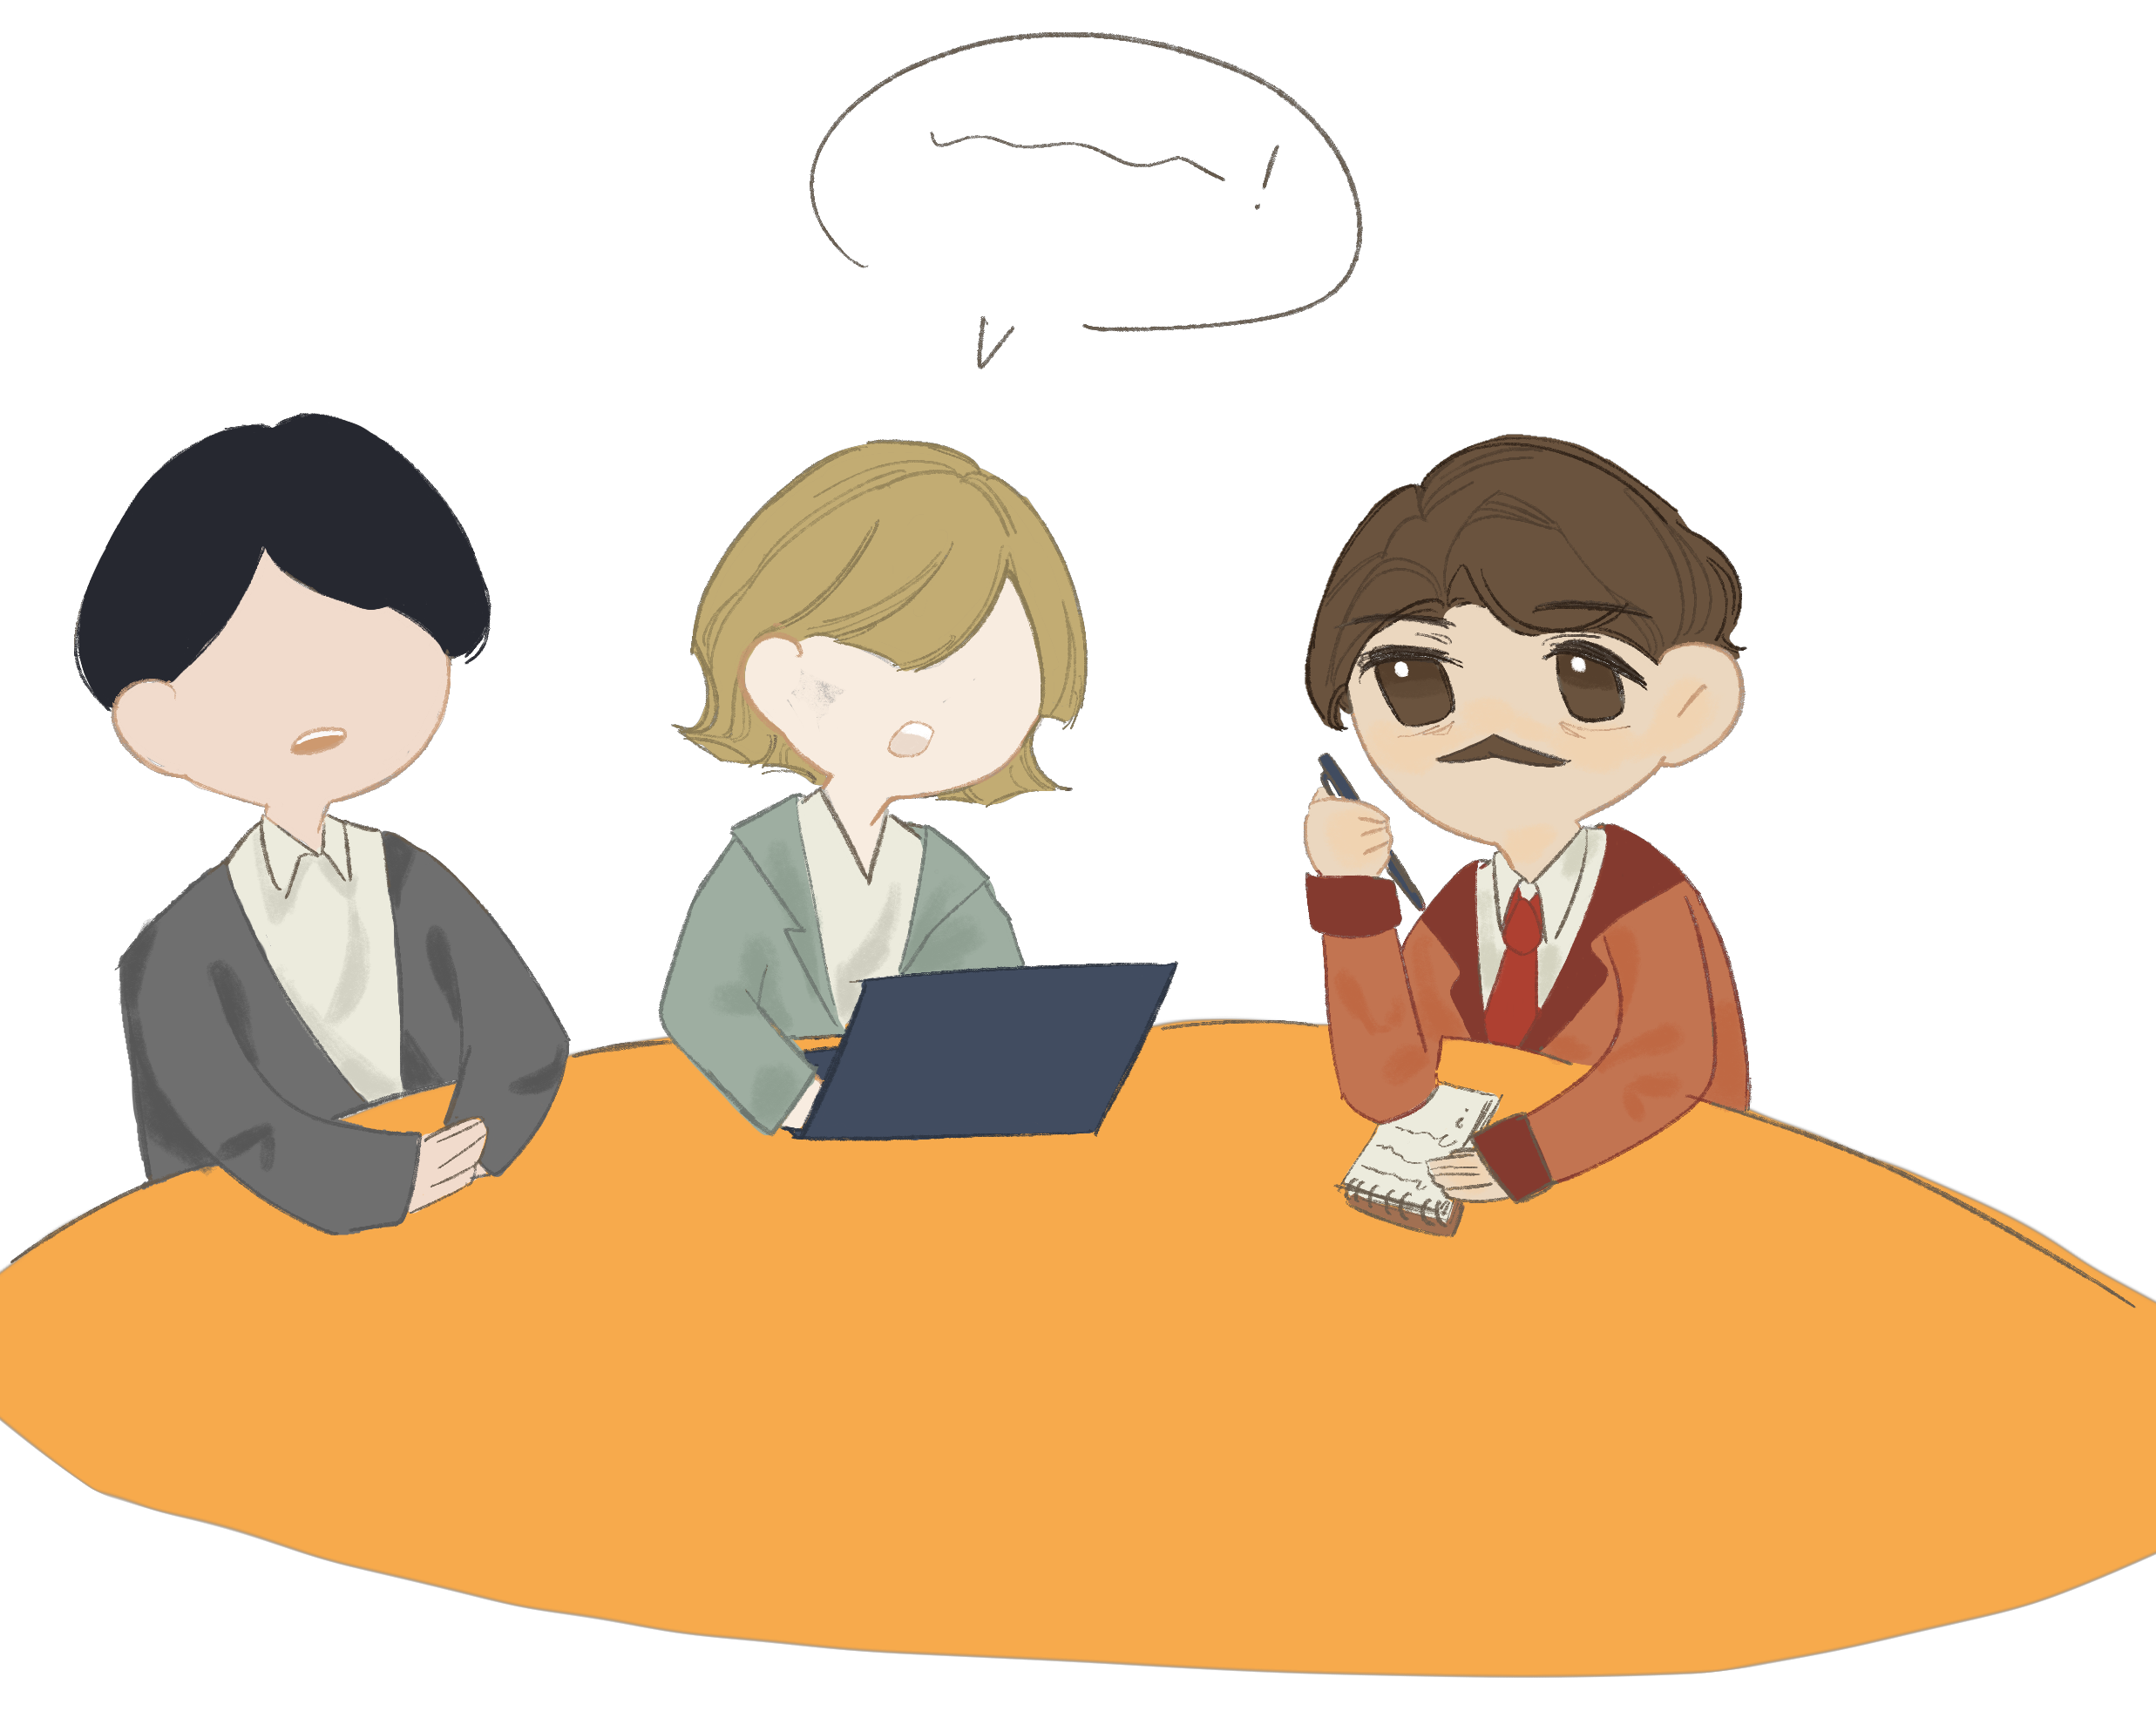
\includegraphics[width=1\linewidth]{xp}
	%		\vspace*{-15pt}
	%	\end{figure}
%	Theo quy định của Hiệp hội Thương gia dành cho những người ngoài, qua lời của bà lão, thám tử có thể đứng dậy bước tới một nơi bất kỳ nào đó trong căn phòng và chỉ được hỏi câu hỏi ``Khoảng cách từ chỗ tôi đứng đến người nói dối gần nhất trong số các anh là bao nhiêu?" cho tất cả những người trong phòng. Sau đó, mỗi người trong số $10$ người ngồi xung quanh bàn sẽ trả lời thám tử, lúc này đã cải trang thành một thương gia muốn gia nhập Hiệp hội. thám tử không được phép đứng lên mặt bàn và tất cả mọi người, kể cả thám tử, đều được phép dùng thước để đo khoảng cách tuỳ ý. Ta cũng được biết rằng ngoài $10$ người và thám tử, trong phòng không còn có người lạ nào khác, hơn nữa $10$ người đều biết rõ ai trong số họ là nói thật và ai trong số họ là nói dối. Em hãy cho biết Xuân Phong có thể sử dụng ít nhất bao nhiêu câu hỏi như trên để biết chắc chắn ai trong số những người ngồi quanh bàn là nói~dối?
%\end{multicols}
%\newpage
%\begingroup
%\AddToShipoutPicture*{\put(115,670){
\includegraphics[scale=1]{../tieude11.pdf}}} 
%\centering
%\endgroup
%\vspace*{35pt}
%
%\begin{multicols}{2}
%	$\pmb{1.}$ Tuấn và Tú cùng tham gia một giải thi đấu cờ vua cùng các bạn học sinh khác trong trường. Hai bạn tổng cộng ghi được $6{.}5$ điểm, trong khi tất cả các bạn học sinh còn lại đều ghi được số điểm bằng nhau. Hỏi có tất cả bao nhiêu học sinh tham gia giải cờ vua đó? (Biết rằng trong giải thi đấu, mỗi người tham gia thi đấu đúng một ván với mỗi người còn lại, ghi được $1$ điểm sau mỗi trận thắng, $0{.}5$ điểm sau mỗi trận hoà và $0$ điểm sau mỗi trận thua).
%	\begin{figure}[H]
	%		\centering
	%		\vspace*{-5pt}
	%		\captionsetup{labelformat= empty, justification=centering}
	%		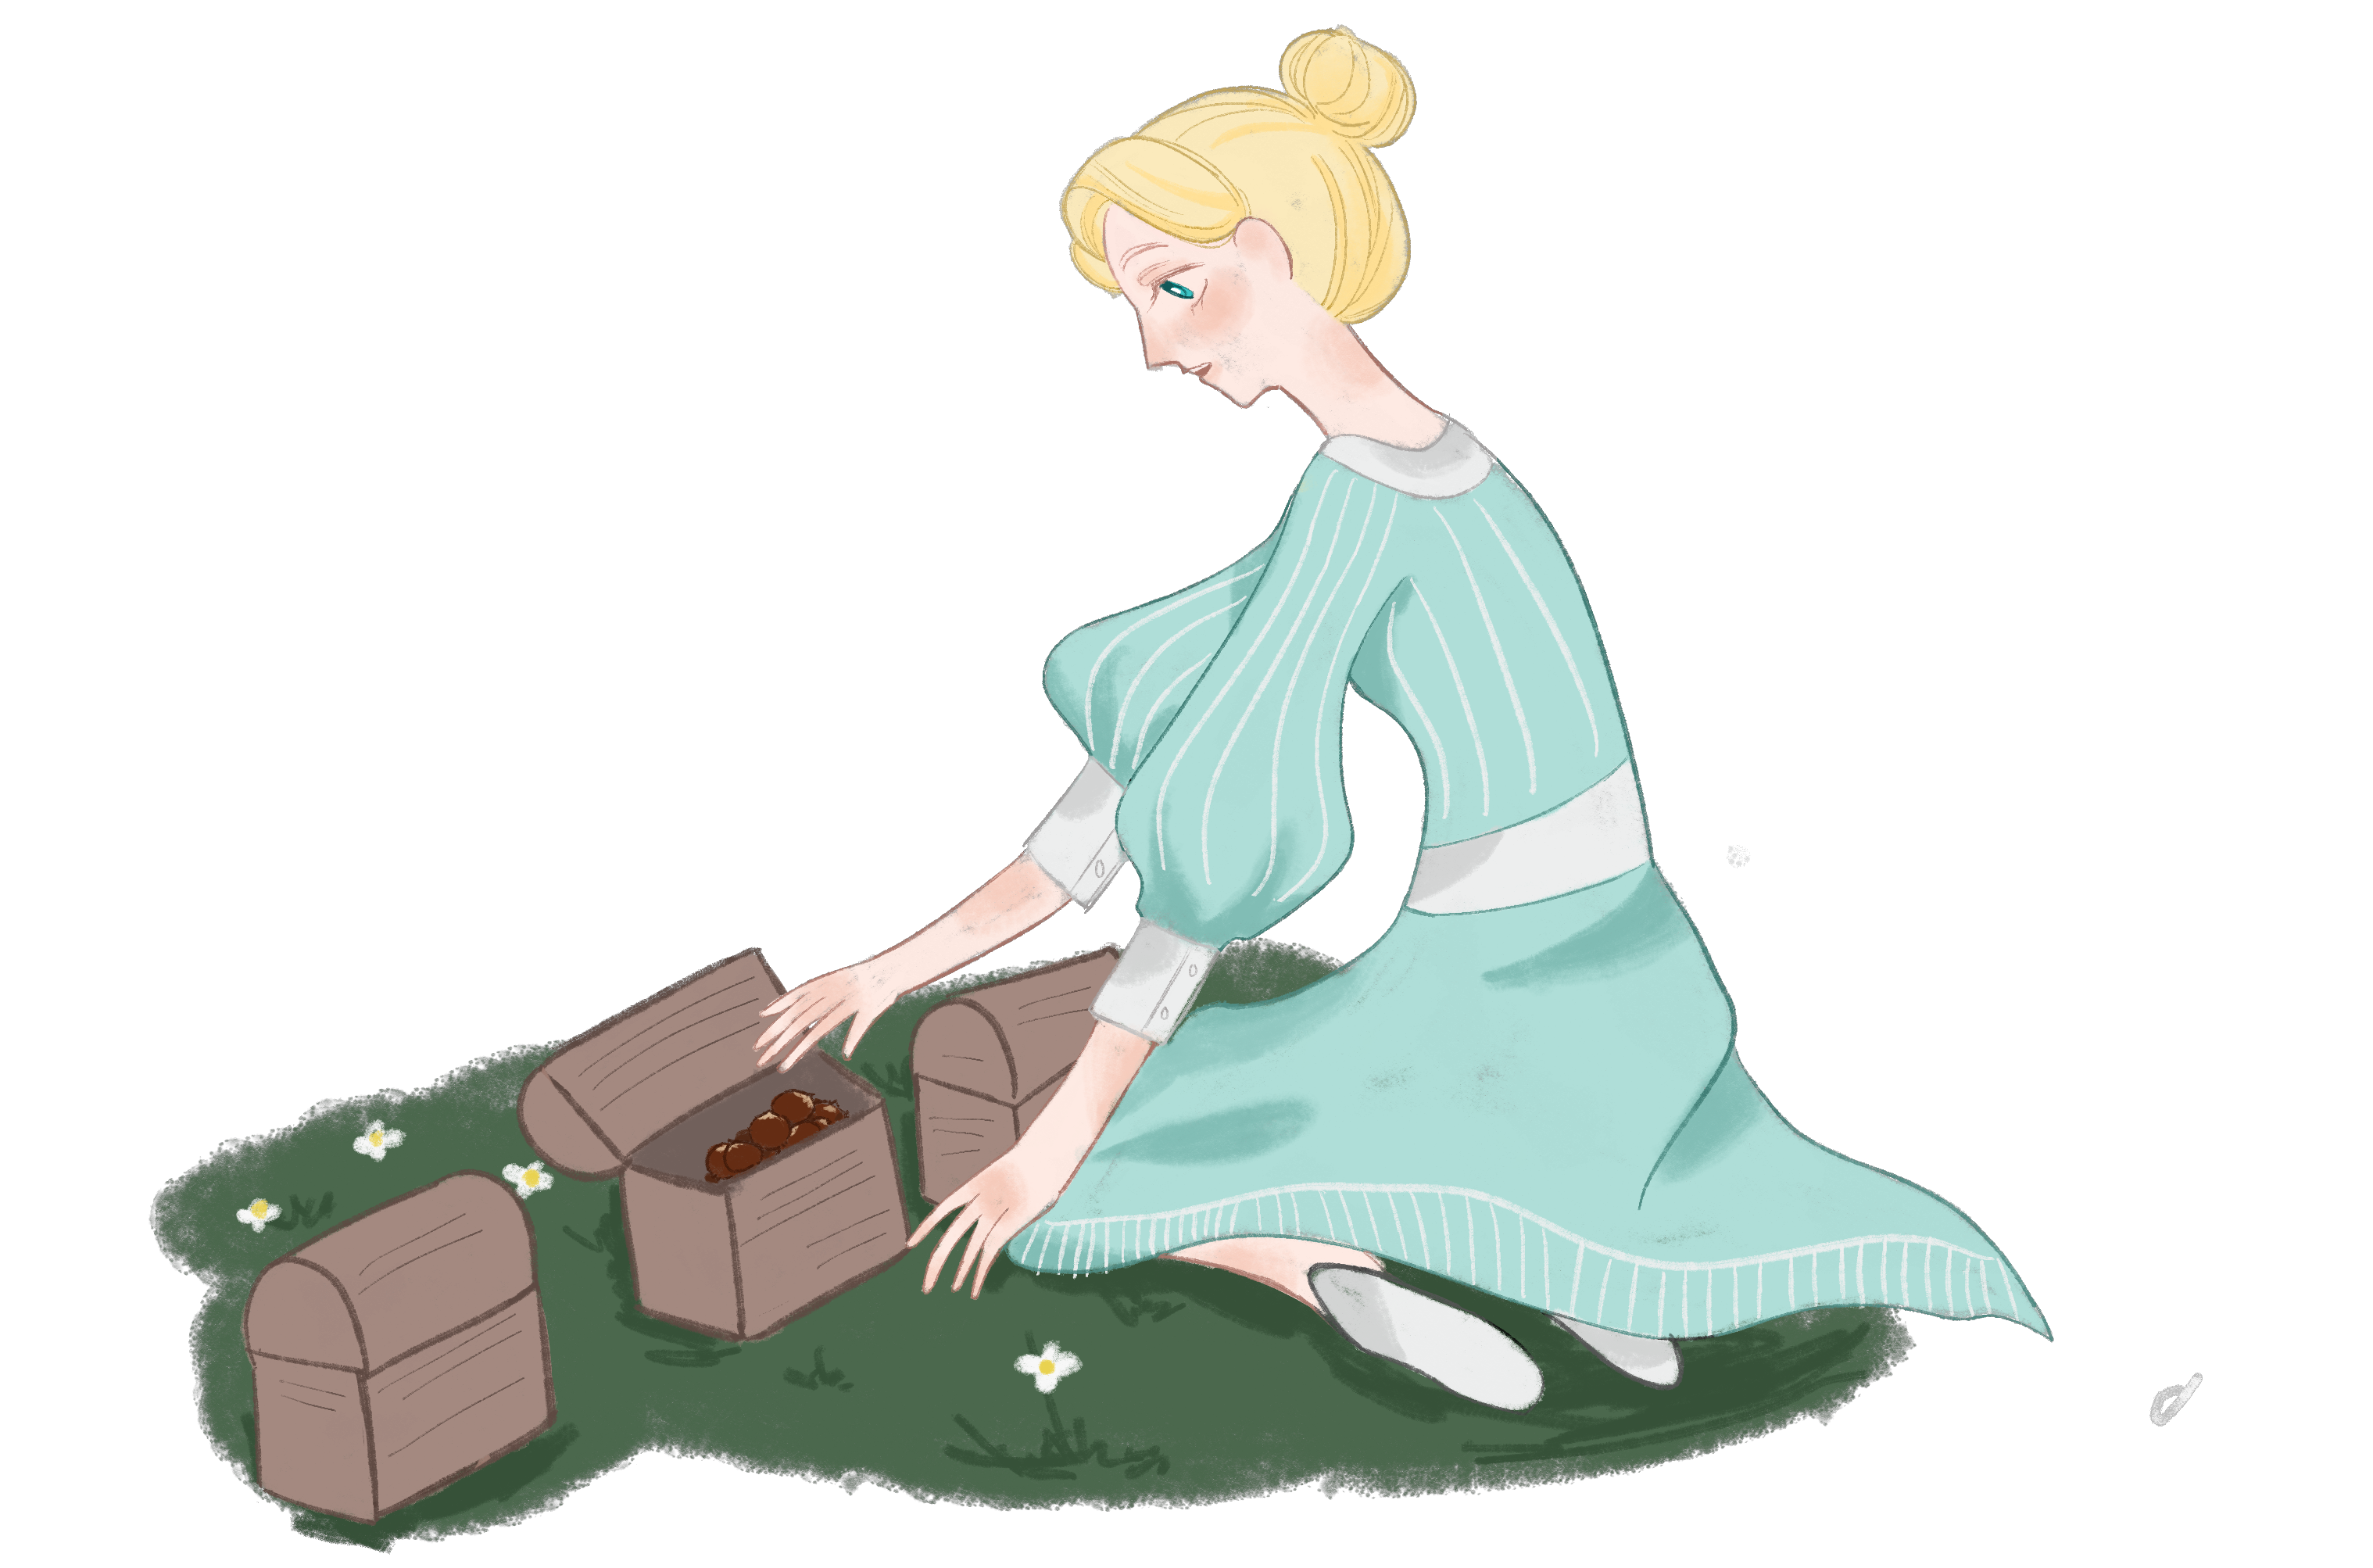
\includegraphics[width=1\linewidth]{Hinh1}
	%		\vspace*{-20pt}
	%	\end{figure}
%	$\pmb{2.}$ 	Lớp $6$A gồm $22$ bạn chia thành hai đội: Xanh gồm các bạn nam và Đỏ gồm các bạn nữ để tổ chức thi tài đối đáp, trả lời thông minh. Đầu tiên, bạn Hoa ở nhóm Đỏ đối đáp với $6$ bạn nam ở nhóm Xanh và giành chiến thắng. Tiếp theo, bạn Mai ở nhóm Đỏ đối đáp với $7$ bạn nam ở nhóm Xanh và cũng giành chiến thắng. Tiếp tục bạn Huệ ở nhóm Đỏ cũng chiến thắng $8$ bạn nam ở nhóm Xanh. Cứ tiếp tục như vậy, cuối cùng bạn Hà ở nhóm Đỏ đã đối đáp thông minh với toàn bộ các bạn nam ở nhóm Xanh và giành chiến thắng chung cuộc. Hỏi trong lớp có tất cả bao nhiêu bạn nam?
%	\begin{figure}[H]
	%		\centering
	%		\vspace*{-5pt}
	%		\captionsetup{labelformat= empty, justification=centering}
	%		
\includegraphics[width=1.01\linewidth]{Hinh2}
	%		\vspace*{-5pt}
	%	\end{figure}
%	$\pmb{3.}$ 	Có bốn chủ doanh nghiệp tới thăm trường học cũ của mình, mang theo một số món quà với dự định sẽ trao tặng cho các học sinh đang học ở đó. Khi tất cả $252$ em học sinh được mời xếp thành một hàng ngang, chủ doanh nghiệp thứ nhất tặng quà cho mỗi em đứng thứ tư trong hàng (các em ở số thứ tự $4,8,12,$ \ldots). Chủ doanh nghiệp thứ hai lại tặng quà cho mỗi em đứng thứ bảy (các em ở số thứ tự $7,14,21$, \ldots). Chủ doanh nghiệp thứ ba trao tặng quà cho mỗi em đứng thứ mười một (các em ở số thứ tự $11,22,33$, \ldots). Chủ doanh nghiệp thứ tư sẽ tặng quà cho các em còn lại. Hỏi có bao nhiêu em học sinh nhận được quà từ mỗi chủ doanh nghiệp?
%	\begin{figure}[H]
	%		\centering
	%		\vspace*{-5pt}
	%		\captionsetup{labelformat= empty, justification=centering}
	%		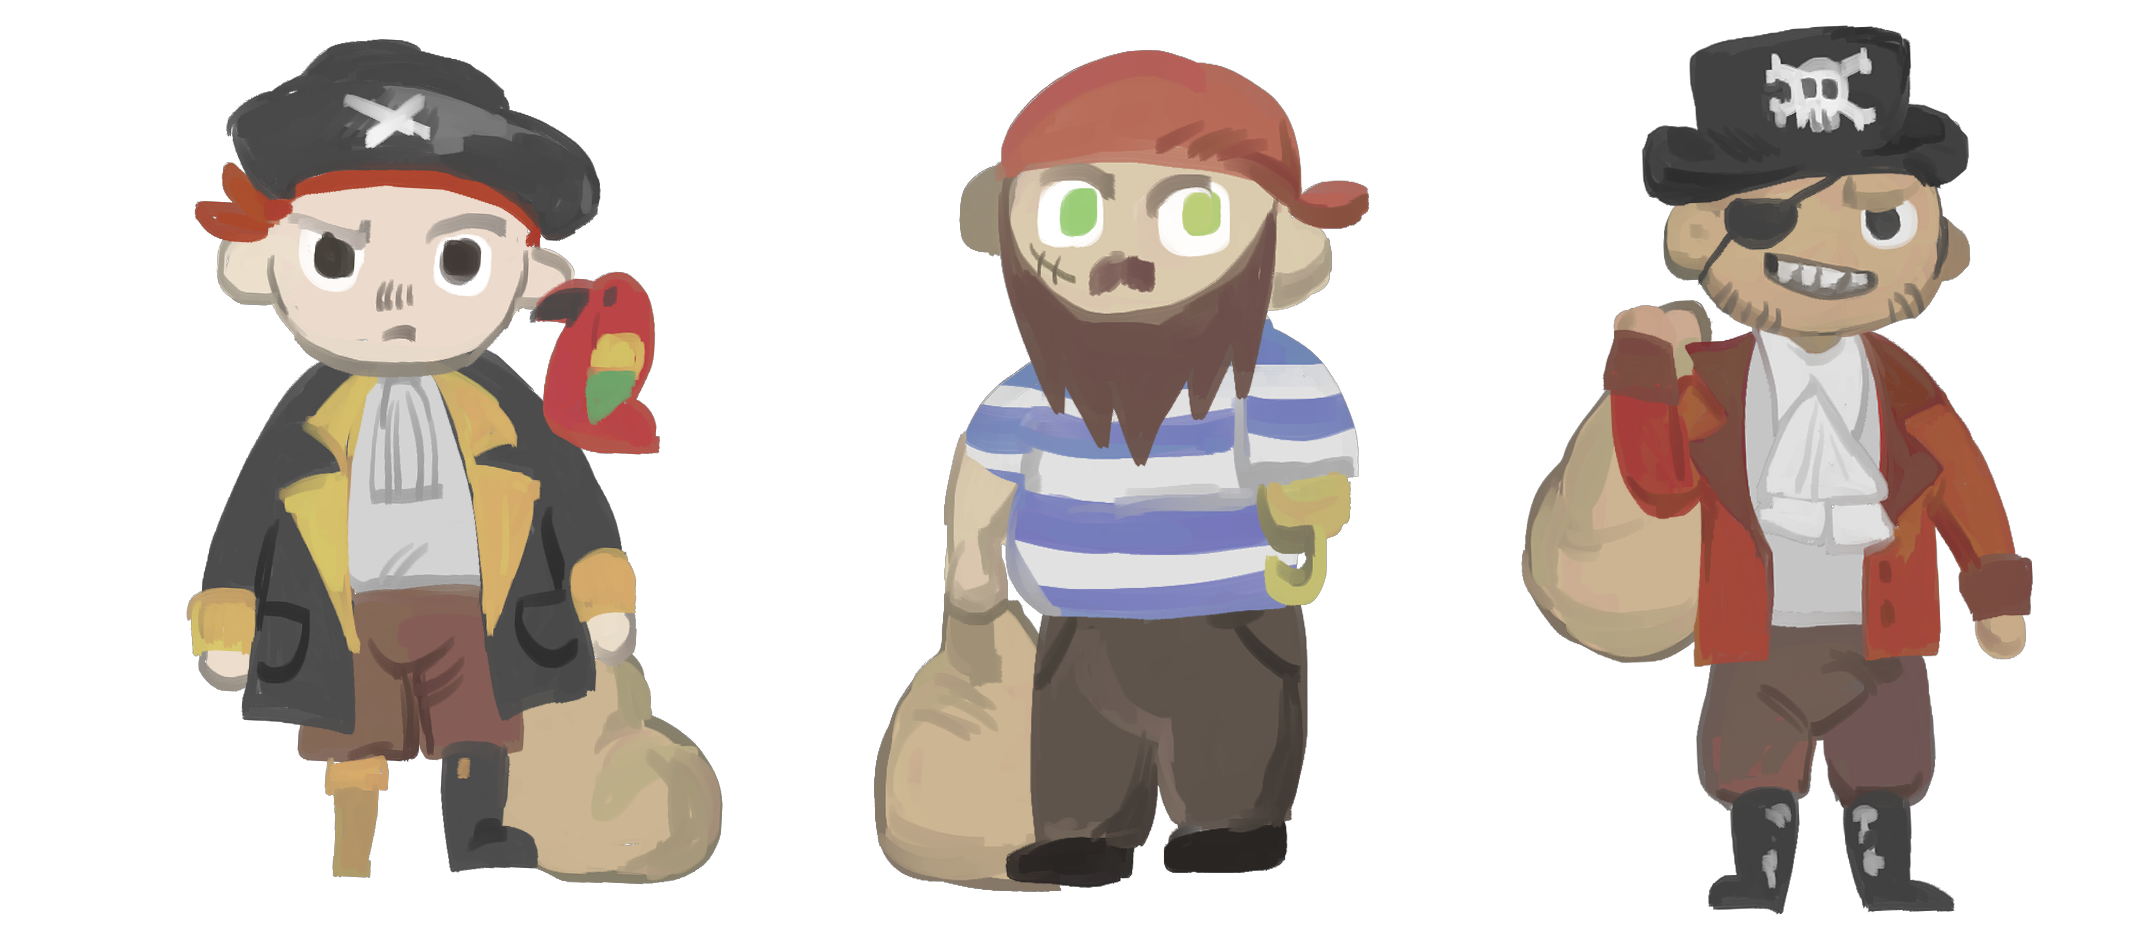
\includegraphics[width=1\linewidth]{Hinh3}
	%		\vspace*{-15pt}
	%	\end{figure}
%	$\pmb{4.}$ 	Có ba nhà tài trợ quyết định giúp đỡ một tạp chí khoa học thường thức với tên gọi là Phi. Nhà tài trợ Quốc trao tặng một khoản tiền tính bằng dollar gồm có $4$ chữ số: $2$ chữ số đứng trước dấu phẩy, và hai chữ số sau dấu phẩy, trong đó số cent lẻ (tức là hai chữ số đứng sau dấu phẩy) bằng với đúng số dollar chẵn (tức là hai chữ số đứng trước dấu phẩy; ta nhớ lại $100$ cent $= 1$ dollar). Nhà tài trợ Minh tặng số tiền với số dollar chẵn lớn hơn $3$ dollar so với số dollar chẵn mà nhà tài trợ Quốc đã tặng nhưng số cent lẻ lại ít hơn $8$ lần số cent lẻ của nhà tài trợ Quốc. Nhà tài trợ Vũ hào phóng đem tặng số tiền bằng $1/7$ tổng số tiền của hai nhà tài trợ Quốc và Minh đã trao cộng lại. Hỏi số tiền ủng hộ của ba nhà tài trợ cho tạp chí Phi là bao nhiêu?
%	\begin{figure}[H]
	%		\centering
	%%		\vspace*{-5pt}
	%		\captionsetup{labelformat= empty, justification=centering}
	%		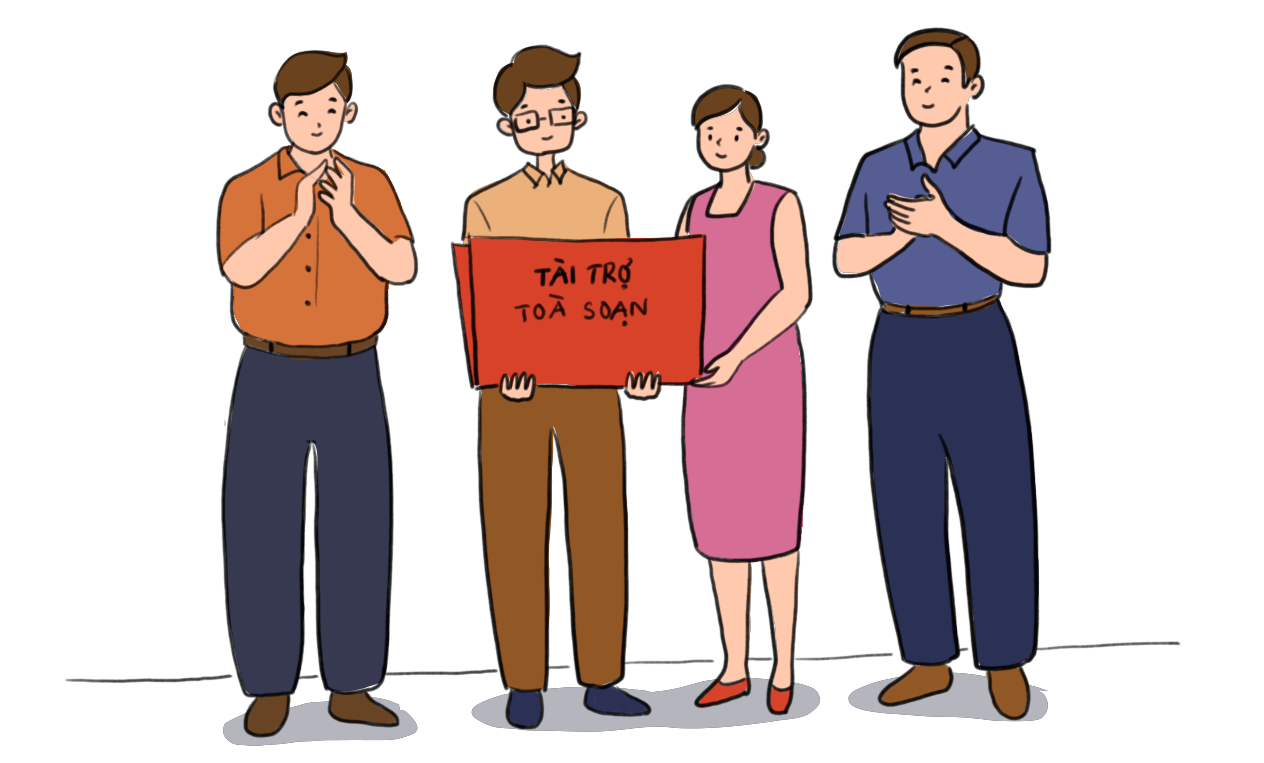
\includegraphics[width=0.8\linewidth]{Hinh4}
	%		\vspace*{-10pt}
	%	\end{figure}
%	\vskip 0.1cm
%	$\pmb{5.}$ 	Trên hòn đảo Ngọc ở giữa một đại dương xanh ngắt có $100$ thổ dân sinh sống, một số người trong họ luôn nói dối, còn những người còn lại luôn nói thật. Mỗi một thổ dân thờ phụng đúng một trong ba vị thần: thần Mặt trời, thần Mặt trăng hoặc thần Đất. Người ta hỏi mỗi thổ dân ba câu hỏi sau đây:
%	\begin{figure}[H]
	%		\centering
	%		\vspace*{-5pt}
	%		\captionsetup{labelformat= empty, justification=centering}
	%		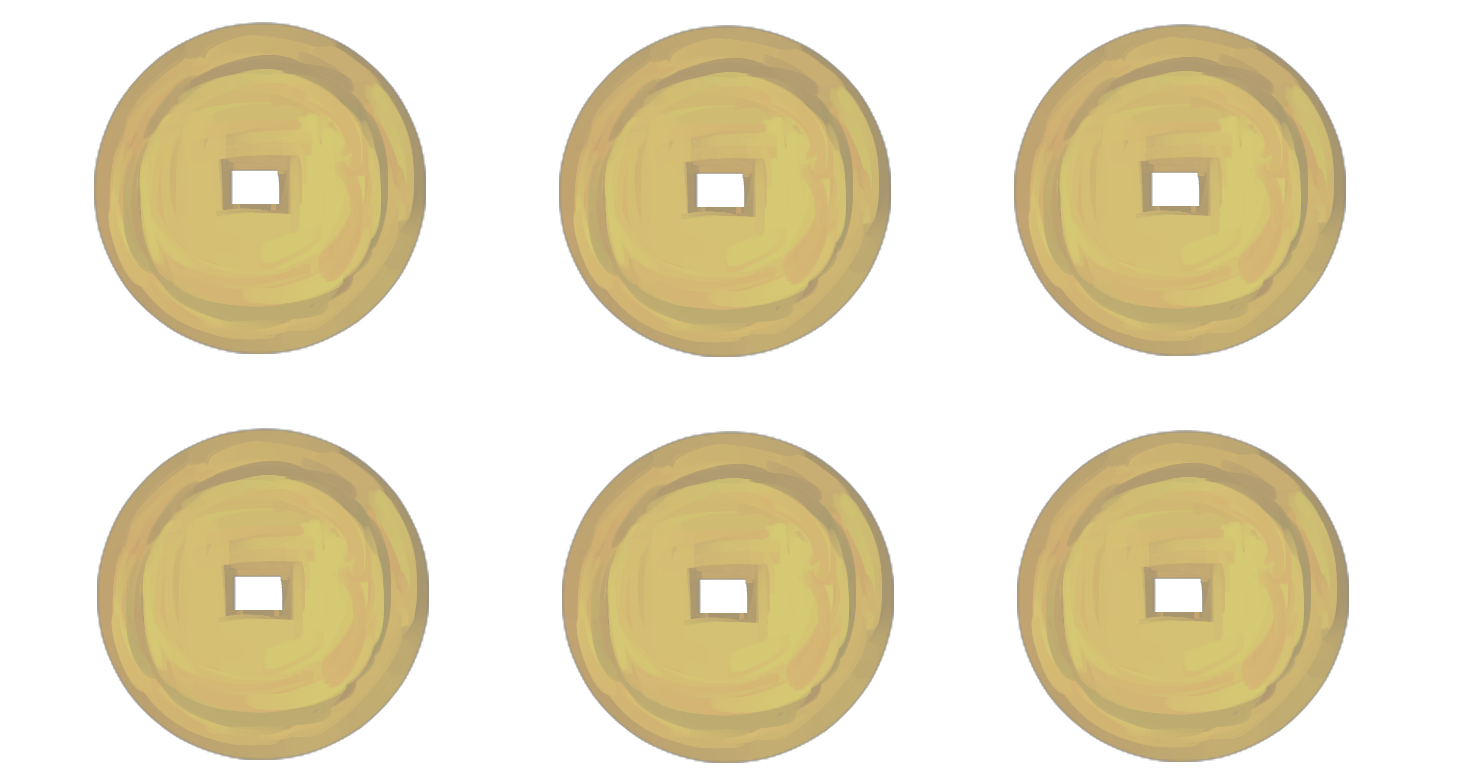
\includegraphics[width=1\linewidth]{Hinh5}
	%		\vspace*{-20pt}
	%	\end{figure}
%	$1.$ Ông (bà) có thờ phụng thần Mặt trời hay không?
%	\vskip 0.1cm
%	$2.$ Ông (bà) có thờ phụng thần Mặt trăng hay không?
%	\vskip 0.1cm
%	$3.$ Ông (bà) có thờ phụng thần Đất hay không?
%	\vskip 0.1cm
%	Có $60$ người trả lời khẳng định ``có" với câu hỏi thứ nhất, $40$ người trả lời khẳng định ``có" với câu hỏi thứ hai và $30$ người trả lời khẳng định ``có" với câu hỏi thứ ba. Hỏi trên đảo Ngọc có bao nhiêu thổ dân nói dối?
%	\vskip 0.1cm
%	$\pmb{6.}$ 	Có $100$ em học sinh được mời tới buổi tổng kết cuối năm học của nhà trường. Các ghế trong phòng họp được xếp ngay ngắn thẳng hàng theo dạng một hình vuông với $10$ dãy ghế, mỗi dãy có đúng $10$ chiếc ghế. Buổi họp phải diễn ra muộn hơn do bị cắt điện, vì thế các em học sinh bắt đầu bàn luận trao đổi với các bạn bên cạnh về kết quả điểm trung bình của mình. Em học sinh nào thấy trong tất cả những bạn ngồi kề sát mình: bên trái, bên phải, đằng sau, đằng trước và theo các đường chéo, chỉ có tối đa một bạn có điểm trung bình cao hơn hoặc bằng điểm trung bình của  mình, sẽ tự coi mình là ``có thành tích".
%	\begin{figure}[H]
	%		\centering
	%		\vspace*{-10pt}
	%		\captionsetup{labelformat= empty, justification=centering}
	%		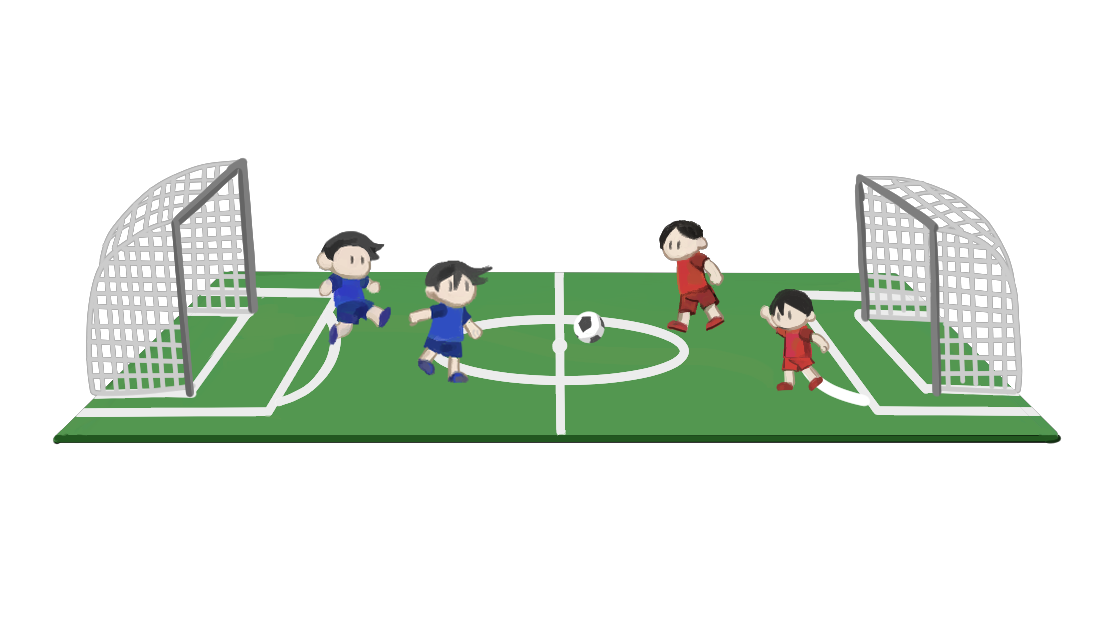
\includegraphics[width=0.85\linewidth]{Hinh6}
	%		\vspace*{-10pt}
	%	\end{figure}
%	Hỏi trong buổi họp đó có thể có tối đa bao nhiêu em học sinh đã tự coi mình là ``có thành tích" trong học tập?
%\end{multicols}
%\vspace*{-10pt}
%{\color{toancuabi}\rule{1\linewidth}{0.1pt}}
%\begingroup
%\AddToShipoutPicture*{\put(114,178){
\includegraphics[scale=1]{../tieude2.pdf}}} 
%\centering
%\endgroup
%\vspace*{75pt}
%
%\begin{multicols}{2}
%	$\pmb{1.}$ Các bạn nam mang kẹo tới lớp để tặng cho các bạn nữ. Bạn Phúc nói rằng mình đã mang tới đúng một nửa tổng số kẹo. Bạn Kiên nói rằng mình đã mang tới đúng một phần ba tổng số kẹo và chỉ chia kẹo của mình cho Mai và Tuyết, hơn nữa Mai được nhiều hơn so với Tuyết là $3$ chiếc kẹo. Em hãy chứng tỏ rằng có một bạn trong số Phúc và Kiên đã \linebreak nhầm lẫn.\\
%	\textit{Lời giải.} Giả sử cả hai bạn Phúc và Kiên đều không nhầm lẫn. Do Phúc không nhầm, nên tổng số kẹo được mang tới lớp phải là số chẵn (gấp $2$ lần số kẹo mà Phúc mang tới). Do Kiên cũng mang tới một số kẹo là số nguyên, bằng $1/3$ của một số chẵn, nên Kiên cũng mang tới một số kẹo là số chẵn. Theo lời của Kiên, số kẹo mà cậu đã tặng cho các bạn nữ là một số lẻ, do số kẹo mà Mai và Tuyết nhận được khác tính chẵn lẻ (hơn kém nhau là $3$ chiếc, mà $3$ là một số lẻ), mà tổng của hai số khác tính chẵn lẻ là một số lẻ. Ta nhận được mâu thuẫn. Suy ra có ít nhất một bạn nam trong số Phúc và Kiên đã nhầm lẫn.
%	\begin{figure}[H]
	%			\centering
	%		\vspace*{-5pt}
	%		\captionsetup{labelformat= empty, justification=centering}
	%		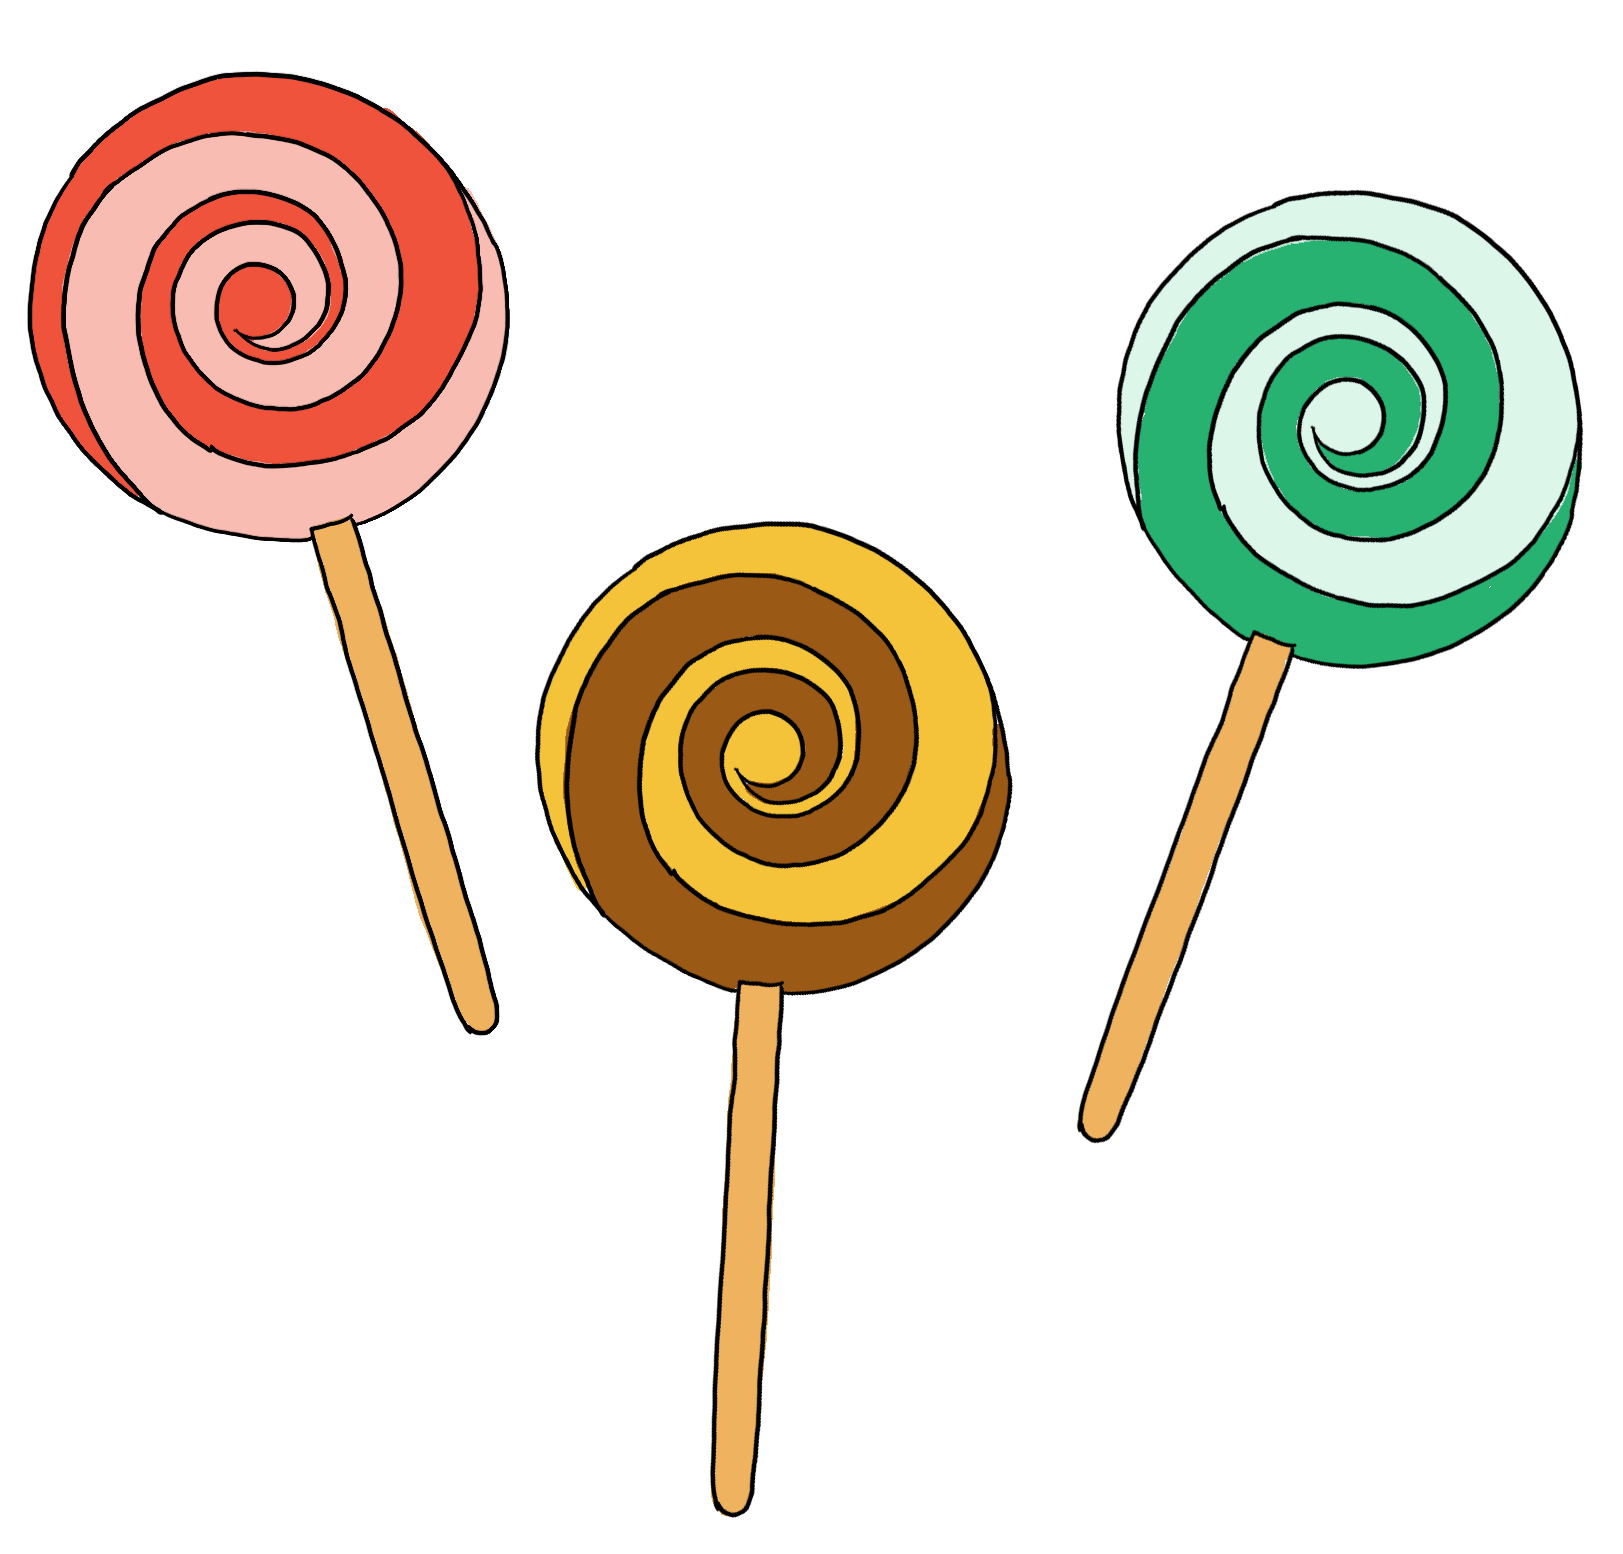
\includegraphics[width=0.6\linewidth]{Pi7_bai1}
	%		\vspace*{-10pt}
	%	\end{figure}
%	$\pmb{2.}$ Ba người thợ cùng đào một chiếc hố. Họ luân phiên lần lượt làm việc, mỗi người làm việc trong một thời gian nhất định. Nếu trong khi một người làm việc hai người còn lại cũng đồng thời đào hố thì hai người này sẽ đào được đúng một nửa hố. Hỏi nếu cả ba người cùng đồng thời đào thì họ sẽ làm nhanh hơn được bao nhiêu lần so với cách làm luân phiên ban đầu?
%	\begin{figure}[H]
	%		\centering
	%		\vspace*{-5pt}
	%		\captionsetup{labelformat= empty, justification=centering}
	%		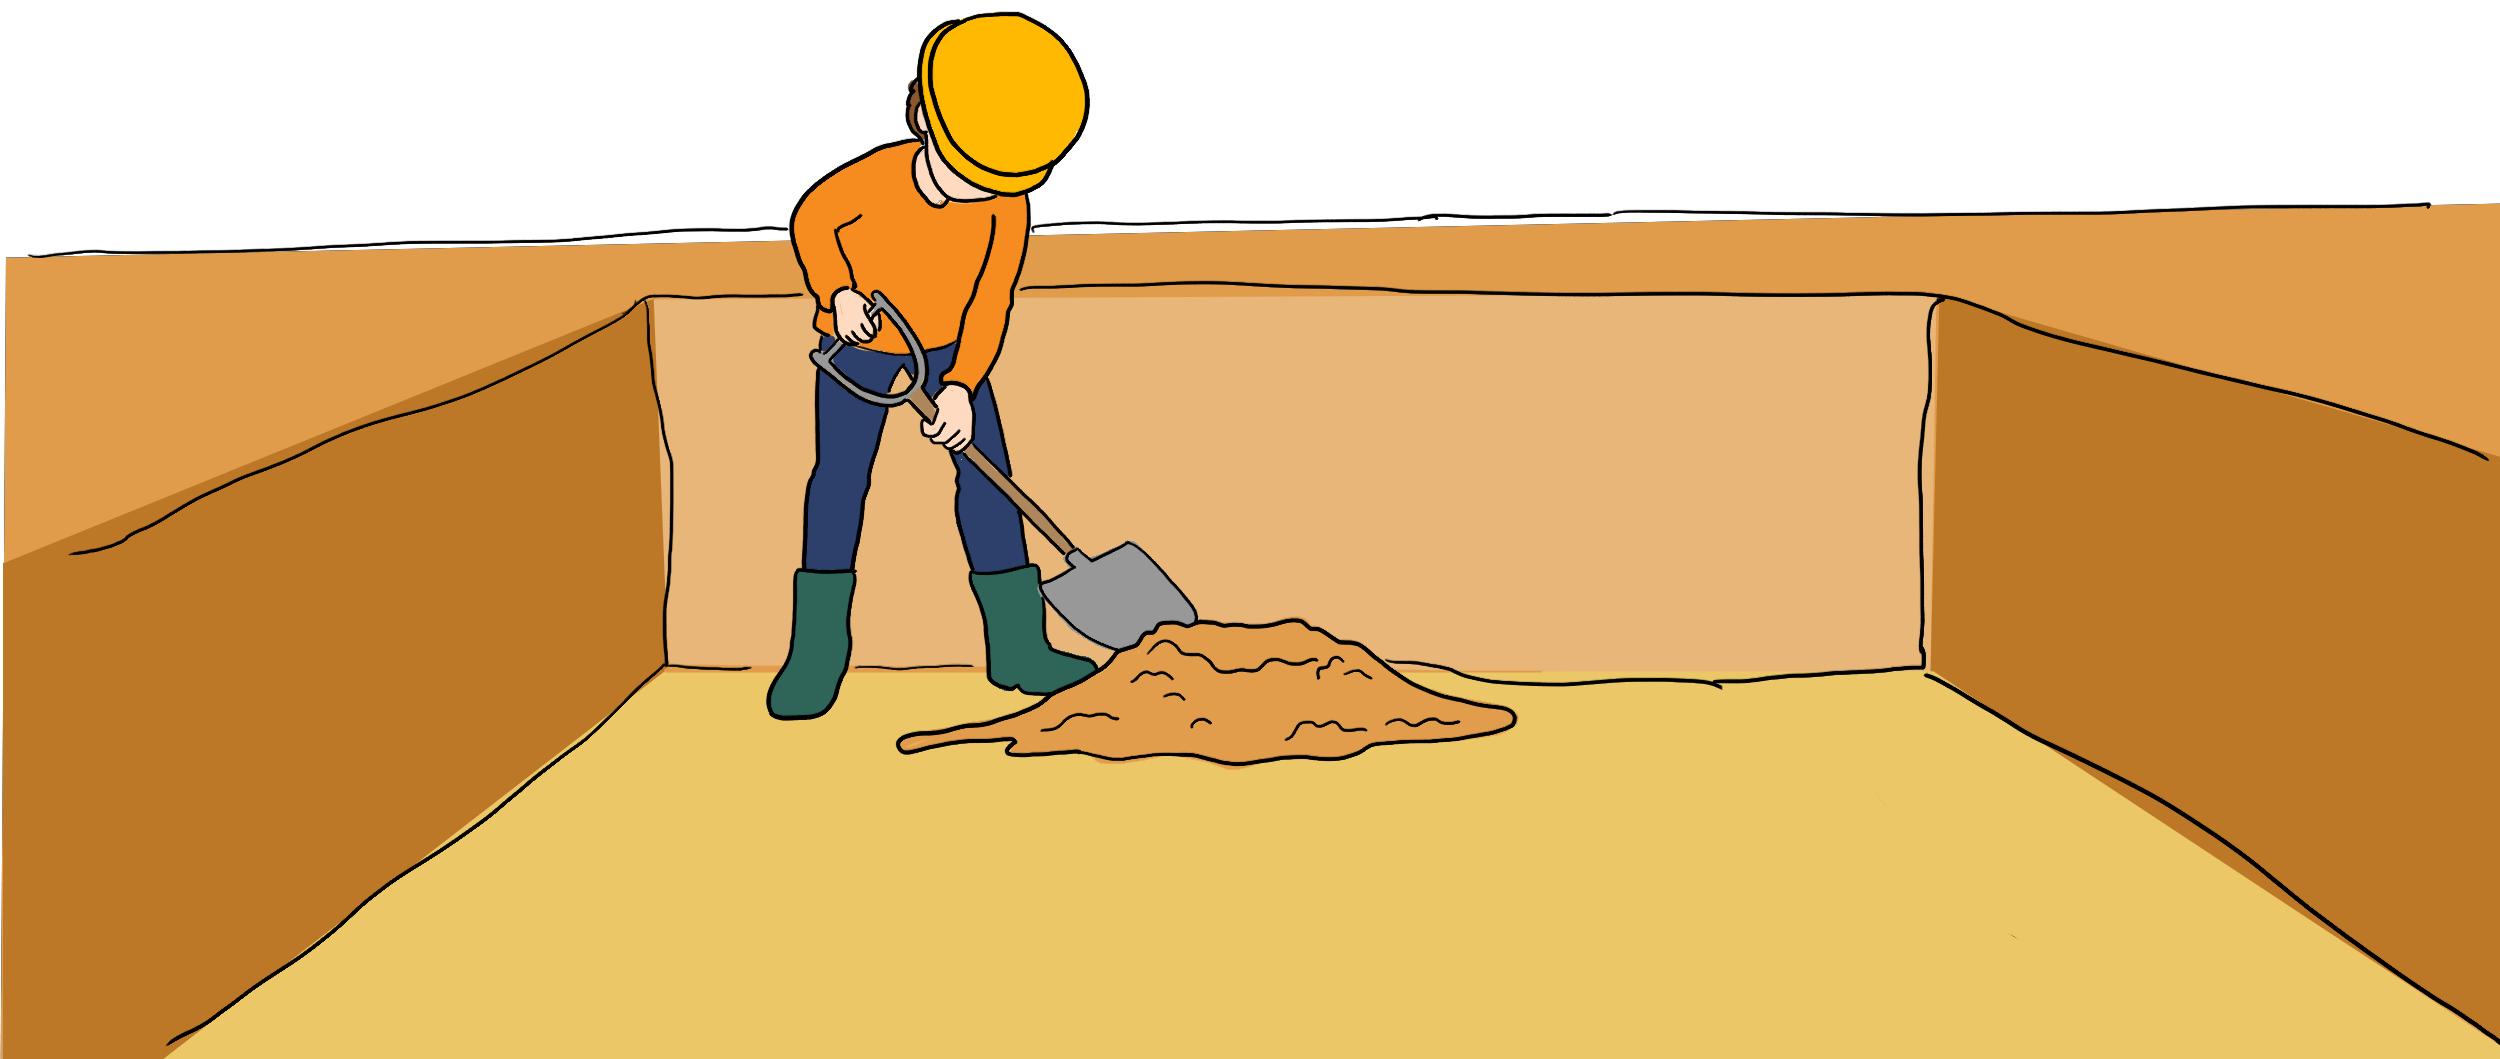
\includegraphics[width=1\linewidth]{Pi7_bai2}
	%		\vspace*{-20pt}
	%	\end{figure}
%	\textit{Lời giải.} 	Giả sử trong thời gian mỗi người đào ở chiếc hố ban đầu, hai người còn lại sẽ đi đào một chiếc hố bổ sung thêm khác. Như vậy khi kết thúc công việc, cùng với chiếc hố ban đầu, họ sẽ đào thêm được $3\cdot 0{.}5 = 1{.}5$ chiếc hố. Do đó, nếu cả ba người cùng làm công việc đào, thì trong cùng số thời gian như ban đầu, họ sẽ đào được $1+1{.}5=2{.}5$ (hố). Vậy, nếu cả ba người cùng đào thì họ sẽ làm nhanh hơn được $2{.}5$ lần so với cách đào luân phiên lần lượt như ban đầu.
%	\vskip 0.1cm
%	$\pmb{3.}$ Ba bạn Gấu, Thỏ và Mèo cùng quyết định xây một con đường từ nhà tới bờ suối với chiều dài $160m$. Các bạn thoả thuận sẽ đầu tư cho dự án mở đường quan trọng này với công sức đều như nhau. Cuối cùng khi dự án hoàn thành, hoá ra bạn Thỏ đã xây được $60$ mét đường, bạn Mèo xây được $100$ mét đường, còn bạn Gấu mải ngủ đông nên không xây được mét nào. Tuy nhiên, Gấu mang tới đóng góp bằng tiền cho dự án là $16$ triệu đồng từ số mật ong bán được của mình. Hỏi hai bạn Mèo và bạn Thỏ cần phải phân chia số tiền cho nhau như thế nào?
%	\begin{figure}[H]
	%		\centering
	%		\vspace*{-5pt}
	%		\captionsetup{labelformat= empty, justification=centering}
	%		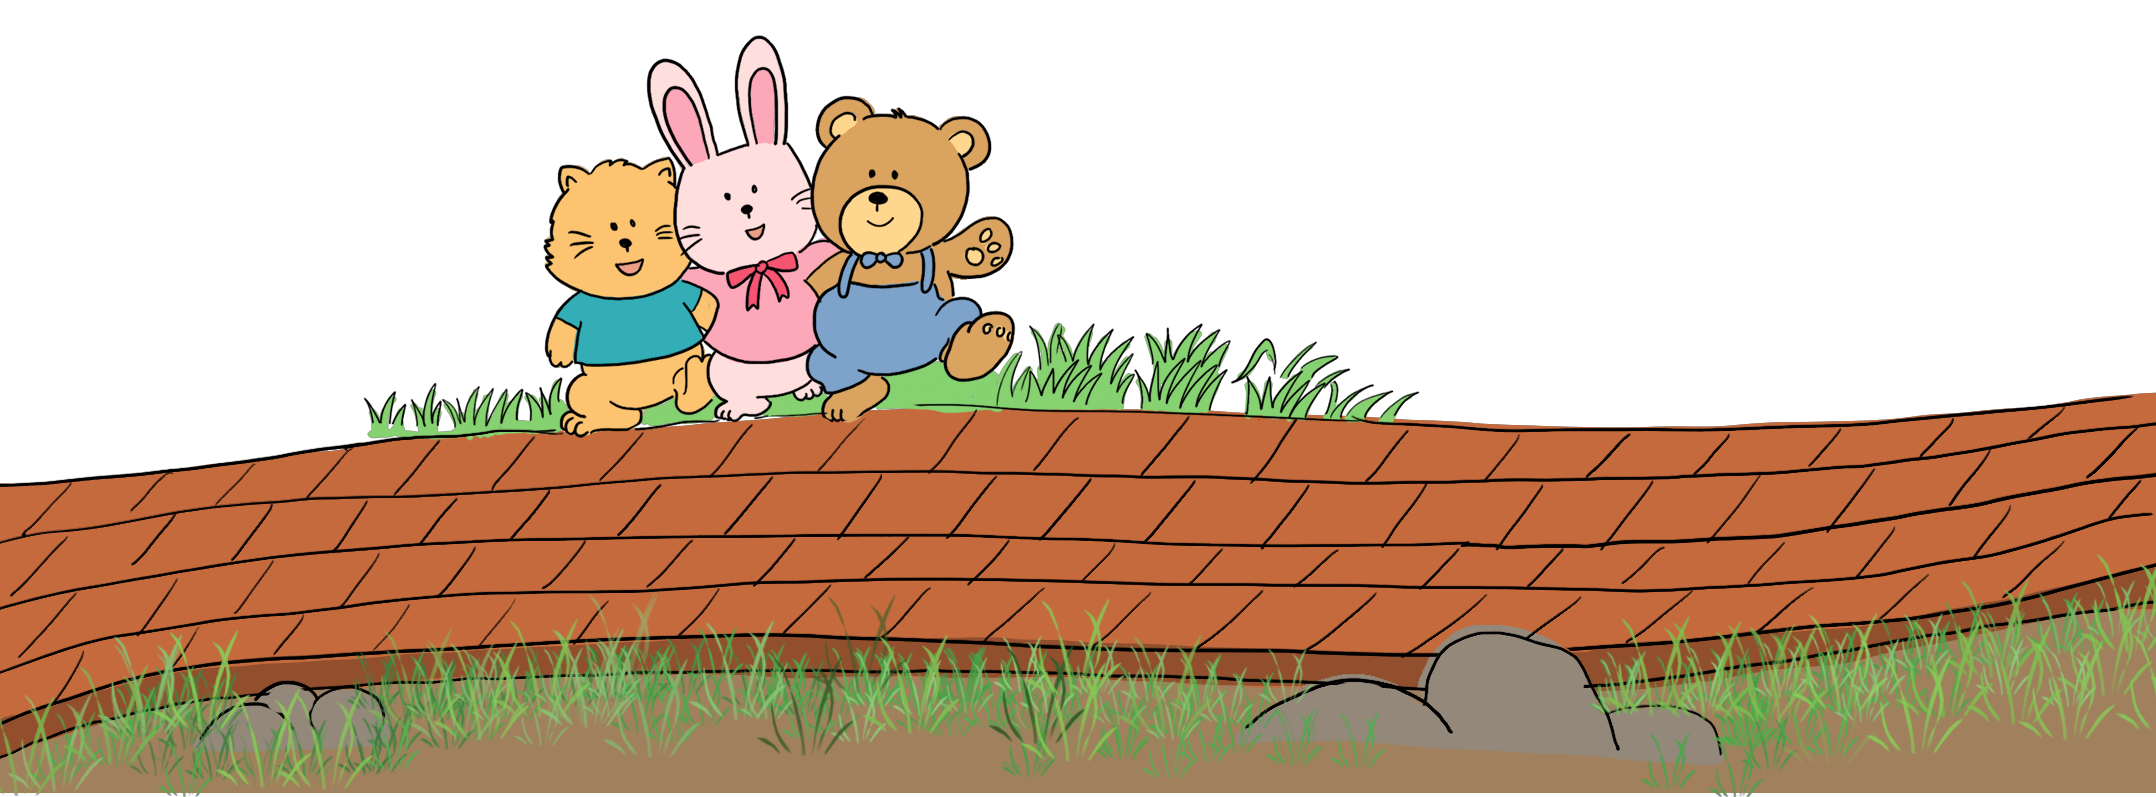
\includegraphics[width=1\linewidth]{Pi7_bai3}
	%		\vspace*{-15pt}
	%	\end{figure}
%	\textit{Lời giải.} 	Mỗi bạn theo kế hoạch phải xây đúng $\dfrac{160}{3} = 53\dfrac{1}{3}$  mét đường. Thỏ xây được $60$ (m) và Gấu xây được $100$ (m). Như vậy bạn Thỏ đã xây thay cho bạn Gấu số mét đường là
%	\begin{align*}
	%		60 - 53 \frac{1}{3} = 6 \frac{2}{3}= \frac{20}{3} \text{ (m)},
	%	\end{align*}
%	còn bạn Mèo đã xây thay cho bạn Gấu số mét đường
%	\begin{align*}
	%		100- 53 \frac{1}{3} = 46 \frac{2}{3}=\frac{140}{3} \text{ (m).}
	%	\end{align*}
%	Vì vậy số tiền mà bạn Gấu mang tới phải chia cho Thỏ và Mèo theo tỷ lệ $2: 14$, tức là Mèo được $14$ triệu đồng, còn Thỏ được $2$ triệu đồng từ số tiền đóng góp công sức của Gấu.
%	\vskip 0.1cm
%	$\pmb{4.}$ Bé Ly phải đi trồng hoa vào một hàng các chậu rất dài đặt thành hàng dọc ở công viên. Bé được giao nhiệm vụ là phải trồng hai loại hoa khác nhau vào hai chiếc chậu nếu giữa hai chậu này có đúng hai chiếc chậu, hoặc đúng ba chiếc chậu, hoặc đúng năm chiếc chậu khác. Hỏi bé Ly phải cần ít nhất bao nhiêu loại hoa để thực hiện được nhiệm vụ?
%	\begin{figure}[H]
	%		\centering
	%		\vspace*{-5pt}
	%		\captionsetup{labelformat= empty, justification=centering}
	%		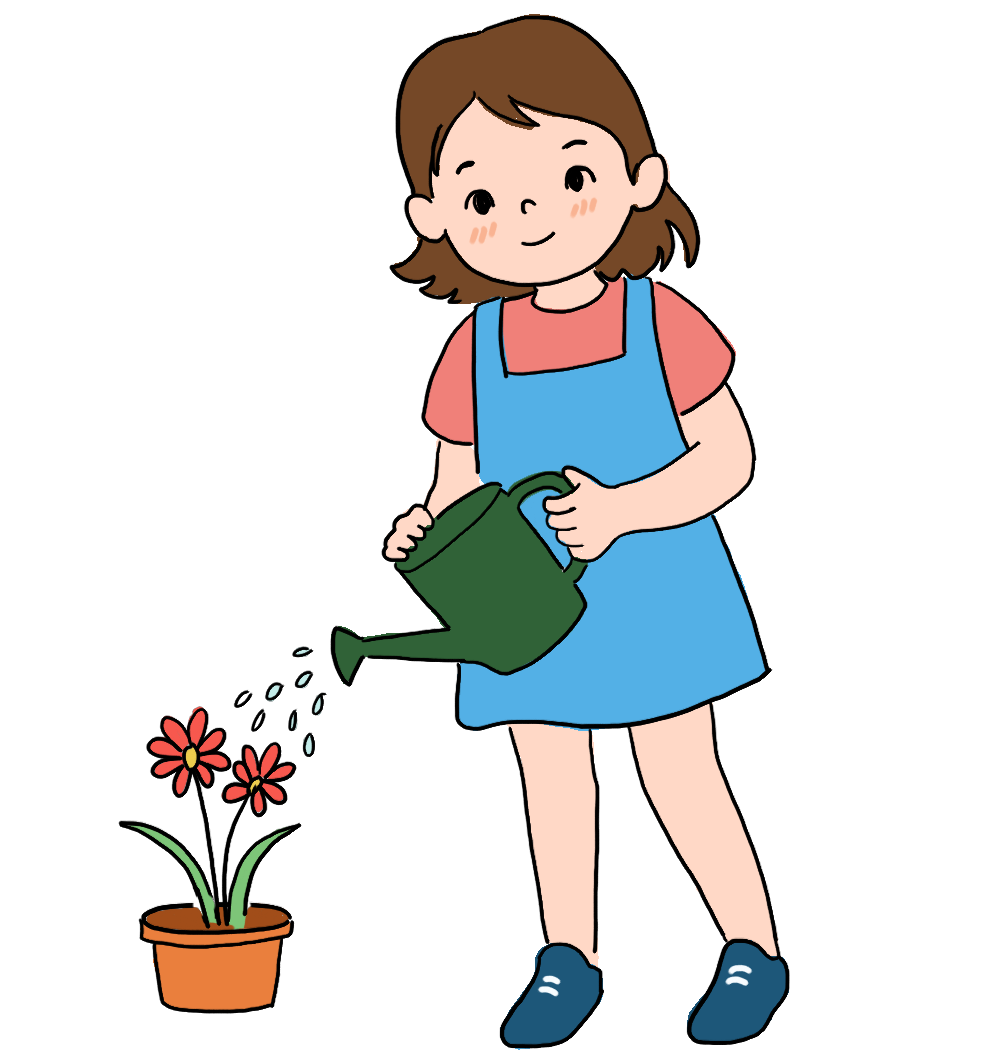
\includegraphics[width=0.45\linewidth]{Pi7_bai4}
	%		\vspace*{-10pt}
	%	\end{figure}
%	\textit{Lời giải.} Trước tiên ta thấy rằng bé Ly có thể chỉ cần $3$ loại hoa là thực hiện được nhiệm vụ. Thật vậy, giả sử Ly có $3$ loại là $A, B, C$. Khi đó nếu Ly trồng $3$ chậu đầu tiên trong hàng bằng loại $A$, $3$ chậu tiếp theo bằng loại $B$, $3$ chậu tiếp loại $C$ và lại $3$ chậu tiếp theo quay lại bằng loại $A$, vv \ldots thì rõ ràng yêu cầu đặt ra được thực hiện. 
%	\vskip 0.1cm
%	Bây giờ giả sử Ly chỉ có $2$ loại hoa là $A$ và $B$. Nếu Ly trồng ở chậu thứ nhất bằng hoa loại $A$ (không mất tính tổng quát), suy ra các chậu có số thứ tự tiếp theo là $4, 5, 7$ phải được trồng bằng hoa loại $B$. Nhưng khi đó giữa hai chậu số $4$ và số $7$ đều được trồng cùng loại hoa $B$ nhưng giữa chúng có đúng hai chậu khác là số $5$ và số $6$, suy ra mâu thuẫn với yêu cầu.
%	\vskip 0.1cm
%	Vậy Ly cần ít nhất $3$ loại hoa để trồng theo yêu cầu đặt ra.
%	 \vskip 0.1cm
%	$\pmb{5.}$ Trước một trận bóng đá giữa hai đội Xóm Đông và Xóm Bắc có $5$ dự đoán kết quả được đưa ra:
%	\vskip 0.1cm
%	$a)$	Sẽ không có tỷ số hoà;
%	\vskip 0.1cm
%	$b)$	Đội Xóm Đông sẽ bị thủng lưới;
%	\vskip 0.1cm
%	$c)$	Đội Xóm Bắc sẽ thắng;
%	\vskip 0.1cm
%	$d)$	Đội Xóm Bắc sẽ không thua;
%	\vskip 0.1cm
%	$e)$	Trong trận bóng sẽ có đúng $3$ bàn thắng được ghi.
%	\vskip 0.1cm
%	Sau khi trận bóng kết thúc, hoá ra chỉ có đúng $3$ dự đoán là chính xác. Vậy trận đấu đã kết thúc với tỷ số như thế nào?
%	\begin{figure}[H]
	%		\centering
	%%		\vspace*{-5pt}
	%		\captionsetup{labelformat= empty, justification=centering}
	%		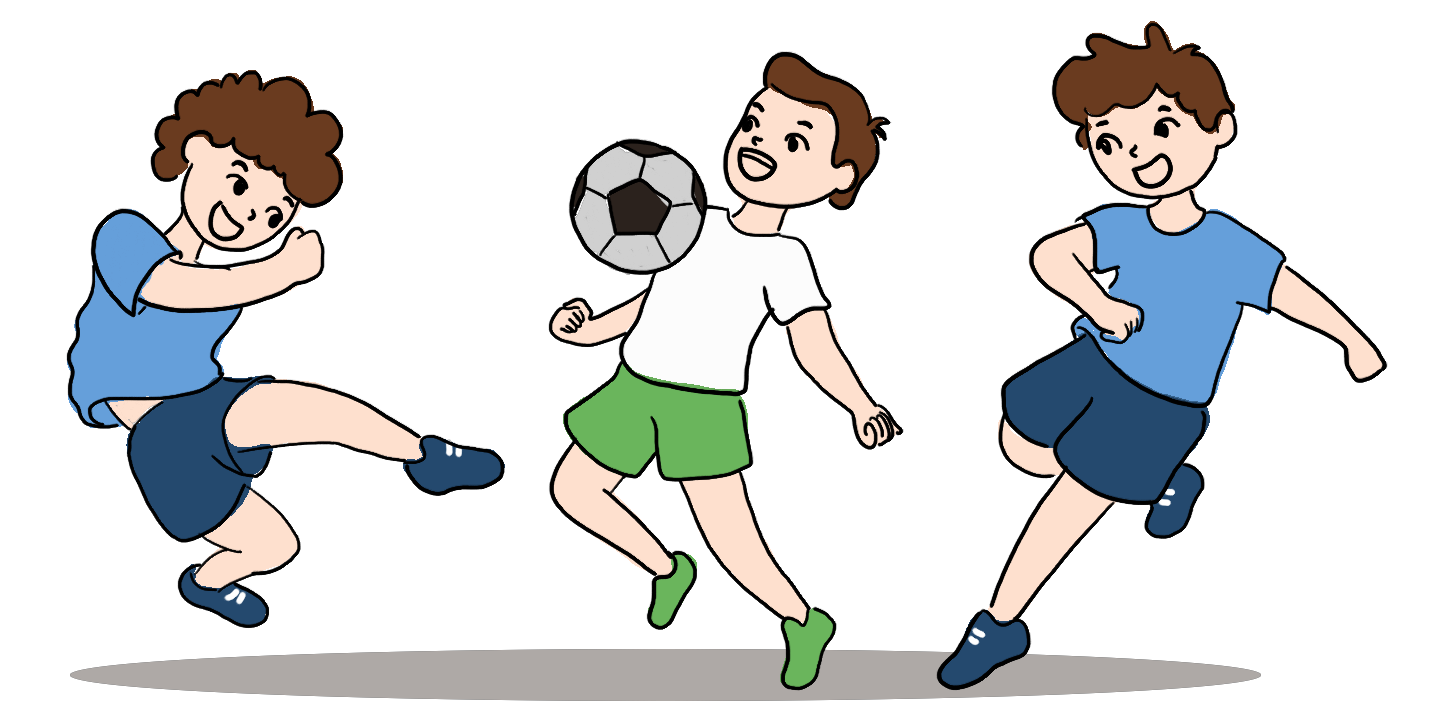
\includegraphics[width=0.85\linewidth]{Pi7_bai5}
	%		\vspace*{-10pt}
	%	\end{figure}
%	\textit{Lời giải.} Giả sử là đội Xóm Bắc thắng. Khi đó $4$ dự đoán $a)$, $b)$ $c)$ và $d)$ đều đúng, mâu thuẫn với điều kiện đặt ra.
%	\vskip 0.1cm
%	Tiếp theo, giả sử trận đấu kết thúc với tỷ số hoà. Khi đó ta lại có các dự đoán $a)$, $c)$ và $e)$ đều sai, điều này cũng mâu thuẫn với điều kiện đã cho.
%	\vskip 0.1cm
%	Vì vậy, trong trận bóng này đội Xóm Bắc đã thua. Khi đó các dự đoán $c)$ và $d)$ đều sai, và $3$ dự đoán còn lại là đúng. Có nghĩa là: trận đấu không có tỷ số hoà, có ít nhất một trái bóng được đưa vào lưới của đội Xóm Đông, và trong trận bóng có đúng $3$ bàn thắng được ghi. Điều đó có nghĩa là trận bóng kết thúc với tỷ số $1:2$ nghiêng về phía đội Xóm Đông.
%	\vskip 0.1cm
%	$\pmb{6.}$ 	Tại trại hè có $20$ em học sinh tham gia trò chơi Điệp viên tí hon diễn ra trong $2$ tuần. Mỗi Điệp viên tí hon sẽ theo dõi và viết báo cáo tỉ mỉ về sở thích cá nhân của $10$ em khác trong số $20$ em này để nộp cho Sở chỉ huy. Em hãy chứng tỏ rằng có ít nhất $10$ cặp Điệp viên tí hon đã theo dõi lẫn nhau và viết báo cáo về nhau.
%	\begin{figure}[H]
	%		\centering
	%		\vspace*{-5pt}
	%		\captionsetup{labelformat= empty, justification=centering}
	%		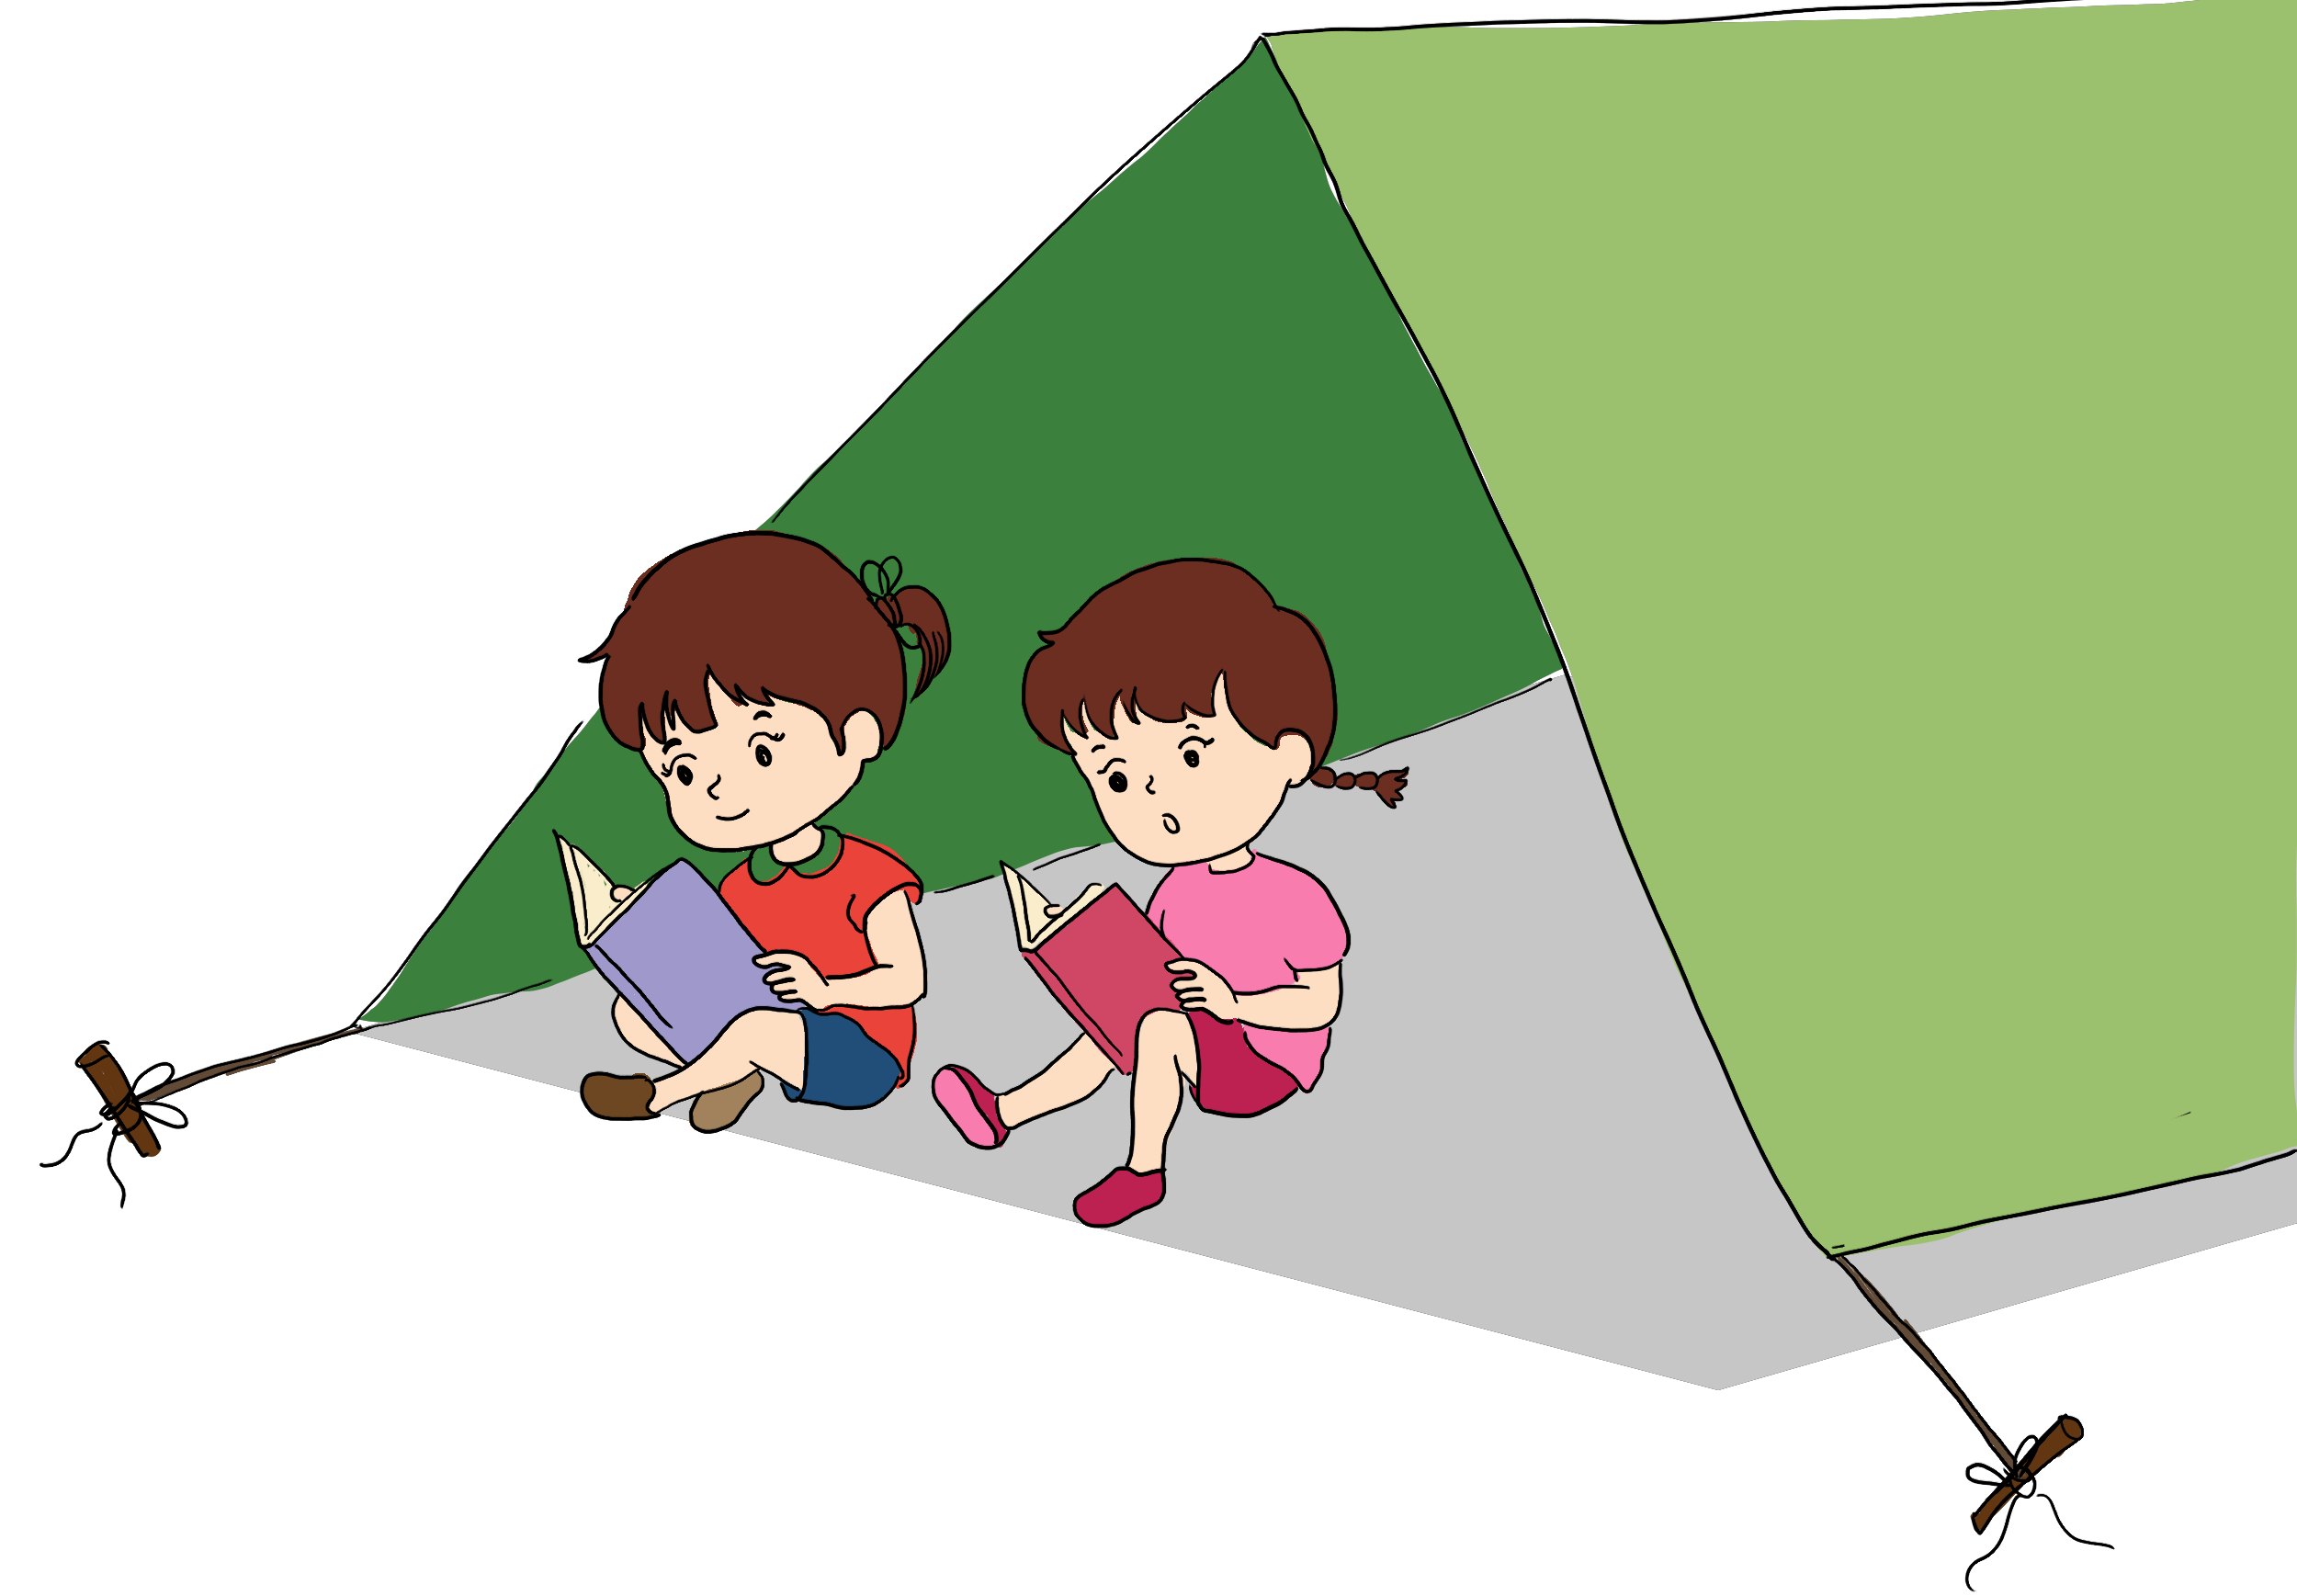
\includegraphics[width=0.75\linewidth]{Pi7_bai6}
	%		\vspace*{-15pt}
	%	\end{figure}
%	\textit{Lời giải.} Số các cặp Điệp viên tí hon là $\dfrac{20\times 19}{2} = 190$ (cặp). Có tất cả $10\times 20=200$ báo cáo được gửi về Sở chỉ huy vào cuối đợt chơi, suy ra phải có ít nhất $10$ cặp Điệp viên mà hai người trong mỗi cặp báo cáo lẫn nhau về Sở chỉ huy.
%\end{multicols}
%
%\newpage
%\begingroup
%\thispagestyle{toancuabinone}
%\blfootnote{$^1$\color{toancuabi}Ottawa, Canada.}
%\AddToShipoutPicture*{\put(60,733){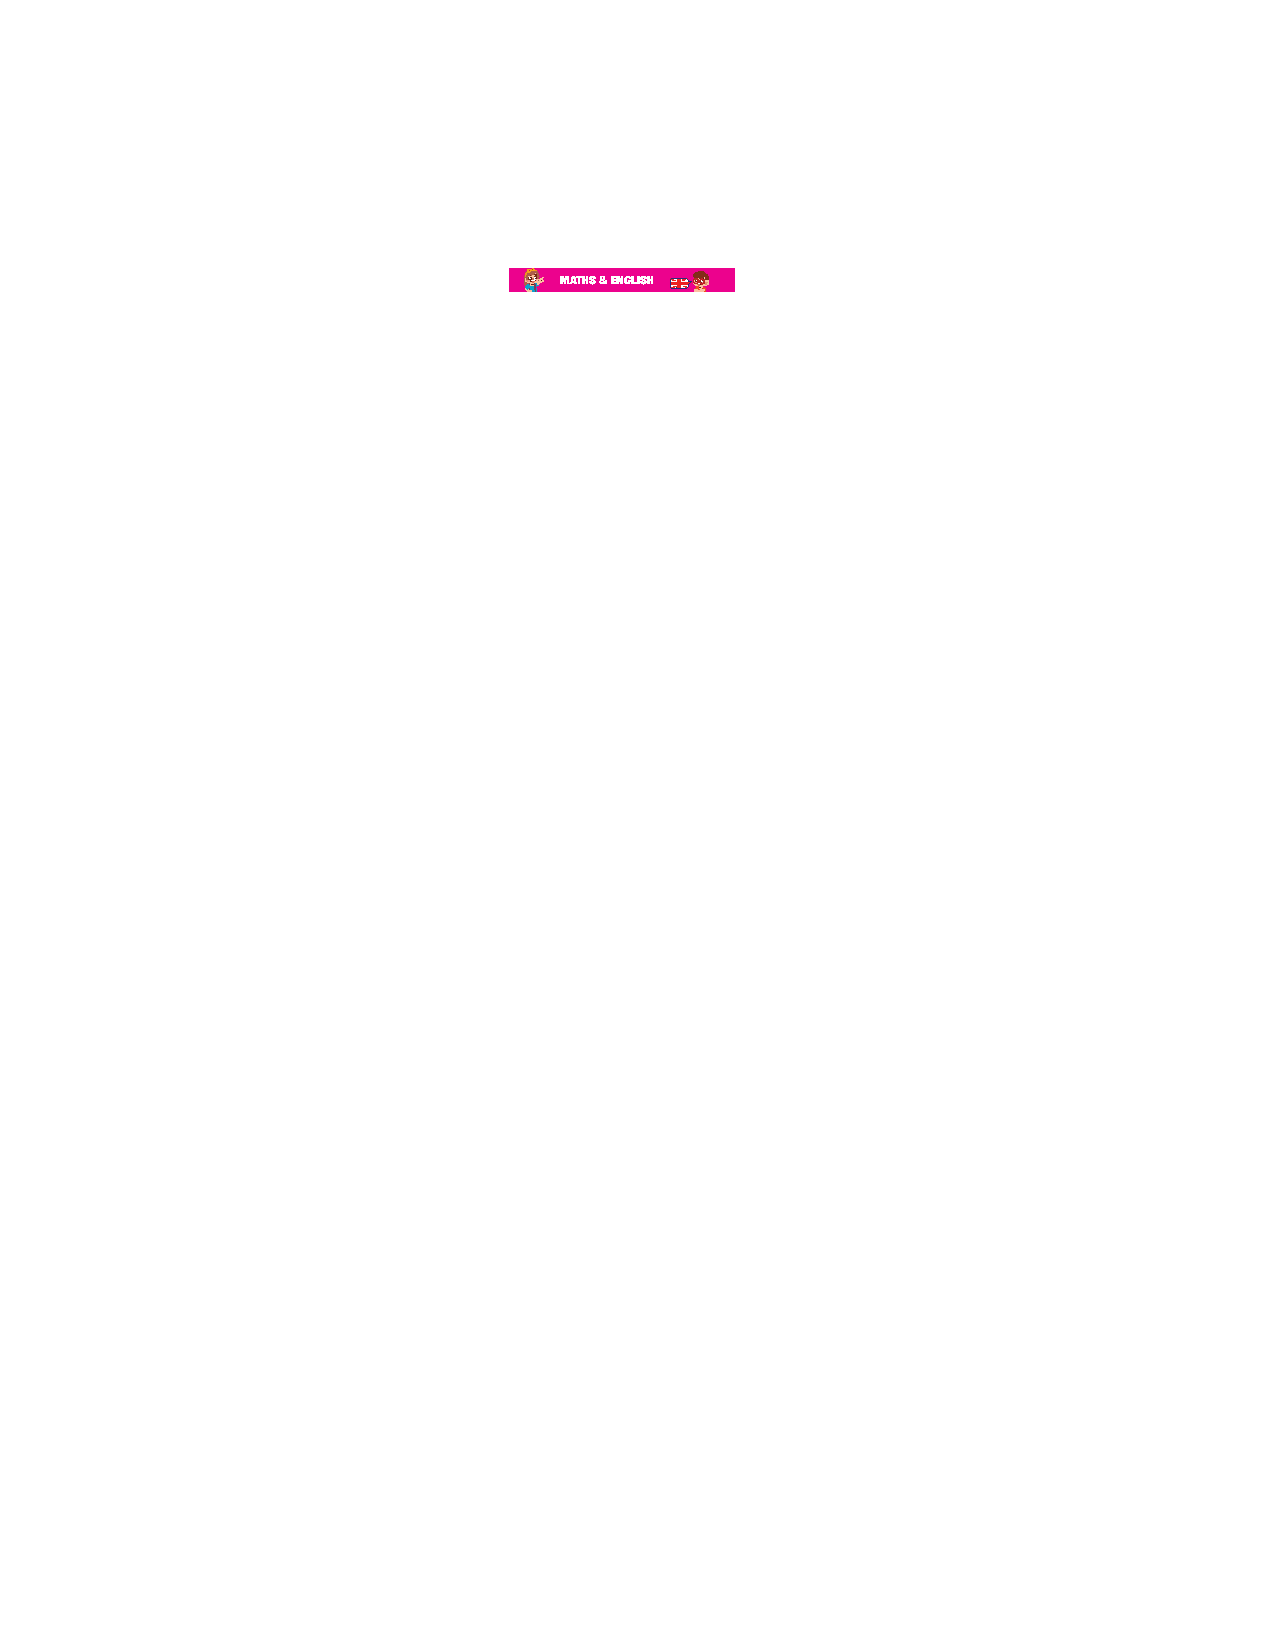
\includegraphics[width=17.2cm]{../mathc.pdf}}}
%%\AddToShipoutPicture*{\put(-2,733){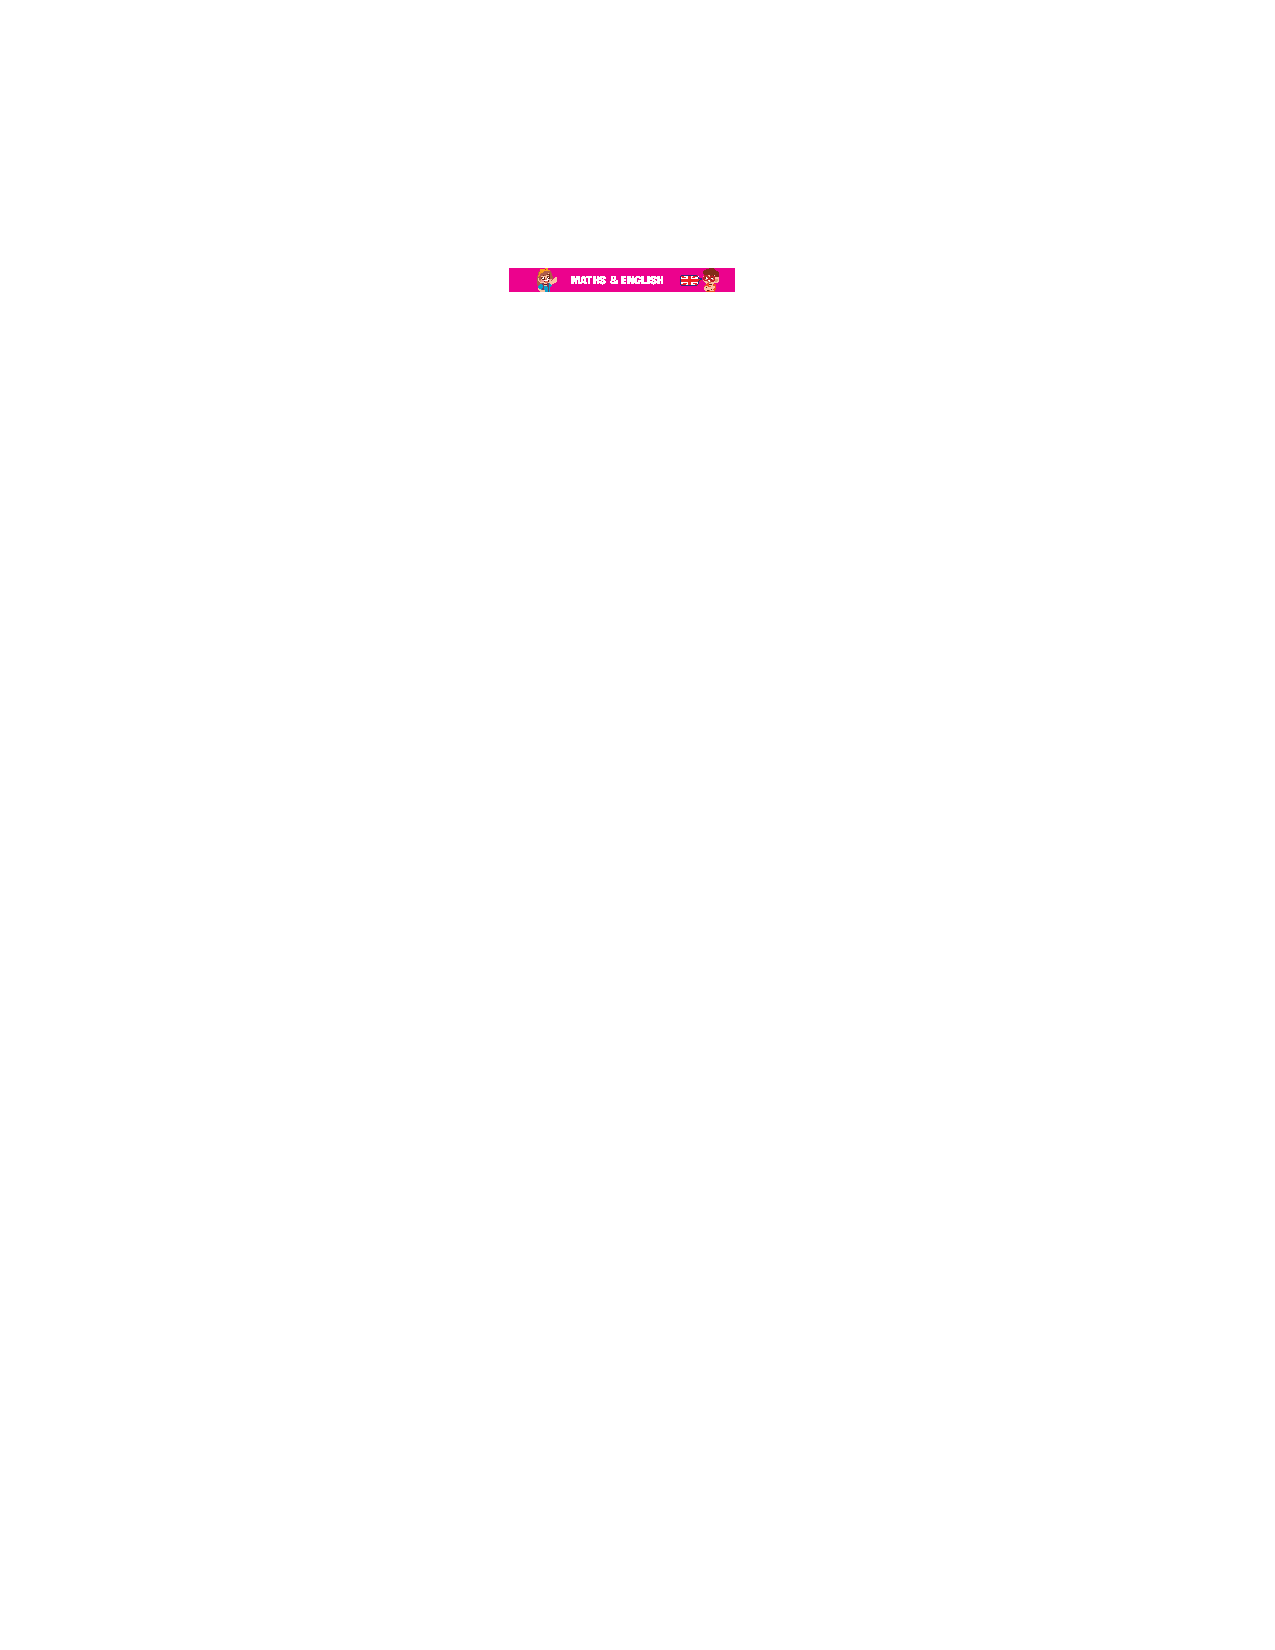
\includegraphics[width=17.2cm]{../mathl.pdf}}} 
%\AddToShipoutPicture*{\put(110,675){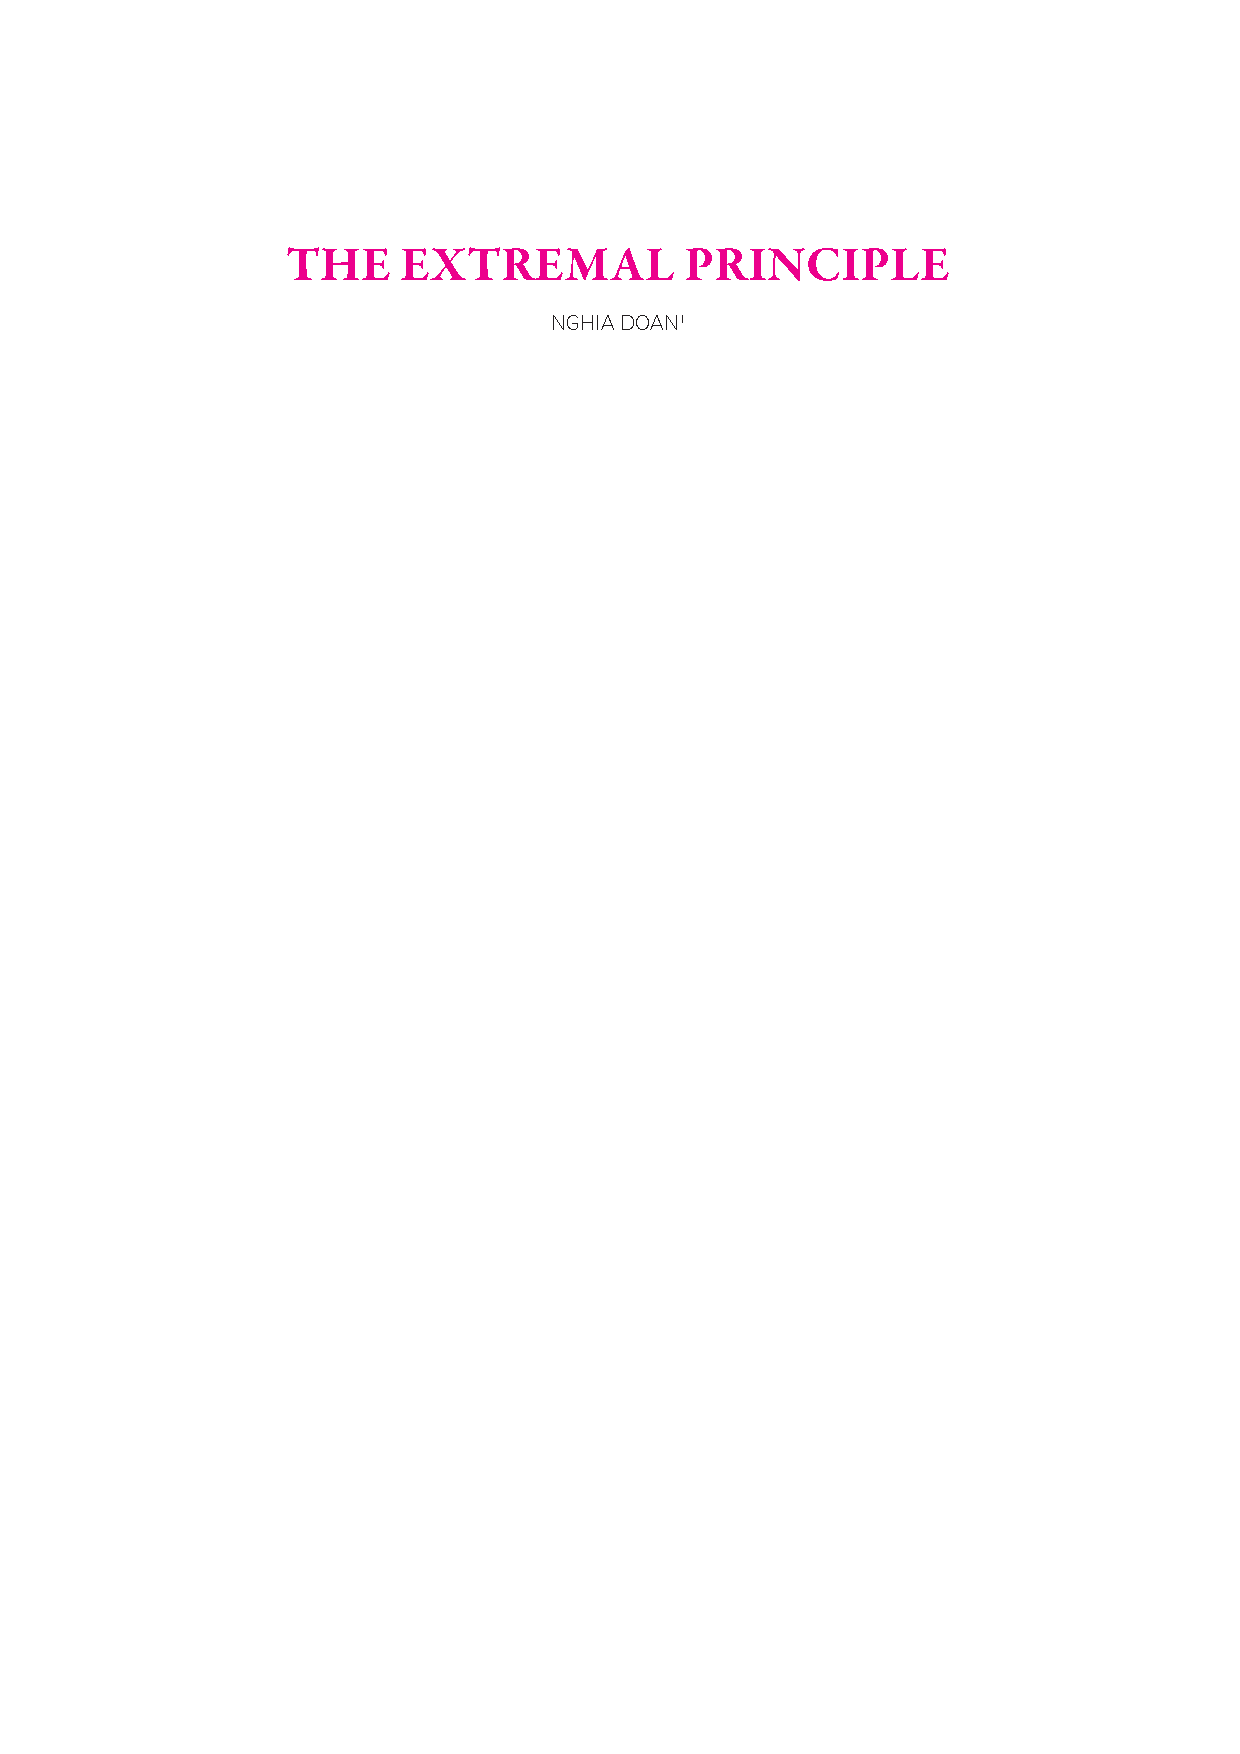
\includegraphics[scale=1]{../tieudeb.pdf}}} 
%\centering
%\endgroup
%\vspace*{35pt}
%
%\begin{multicols}{2}
%	In this article, we discuss the Extremal Principle and its applications.
%	One of the simplest forms of the principle is as follow:
%	``in a finite set of numbers, there is a number with minimal value,
%	i.e. it is smaller than or equal to any other number in the set.
%	Similarly there is a number with maximal value,
%	i.e. it is larger than or equal to any other number in the set."
%	\vskip 0.1cm
%	\textit{Proof by contradiction} is an extremely useful tool when combining with the Extremal Principle,
%	as you will see in below examples.
%	\vskip 0.2cm
%	\PIbox{{\color{toancuabi}\textbf{\color{toancuabi}\color{toancuabi}\color{toancuabi}\color{toancuabi}Example} (Dancing at a party)}
	%			At a party no boy danced with all the girls,
	%			but each girl dances with at least one boy.
	%			Prove that there are two pairs of girl--boy $(g_1, b_1)$ and $(g_2, b_2)$
	%			who danced with each other but $g_1$ did not dance with $b_2$
	%			and $g_2$ did not dance with $b_1.$}
%	\vskip 0.2cm
%	\textit{Solution.}
%		Let $b_1$ be \textit{the boy who danced with the maximum number of girls.}
%		Then there is a girl $g_2$ who he did not danced with.
%		For $g_2$ there is a boy $b_2$ that $(g_2,b_2)$ danced together.
%		Among the girls who danced with $b_1$ there is at least one $g_1$ who did not danced with $b_2,$
%		otherwise $b_2$ danced with $g_2$ and all the girls that $b_1$ danced with,
%		meaning $b_2$ danced with more girls than $b_1,$ contradicting with the choice of $b_1.$
%	\vskip 0.2cm
%	\PIbox{{\color{toancuabi}\textbf{\color{toancuabi}\color{toancuabi}\color{toancuabi}\color{toancuabi}Example} (Infinity by contradiction)}
	%			$\Omega$ is a set of points on the plane.
	%			Every point in $\Omega$ is a midpoint of two points in $\Omega$.
	%			Show that $\Omega$ is infinite set.}
%	\vskip 0.2cm
%	\textit{Solution.}
%	Suppose that $\Omega$ is a finite set.
%	According to the Extremal Principle,
%	\textit{there exists two points $A, B \in \Omega,$ such that the distance $AB$ is maximal.}
%	\vskip 0.1cm
%	Now, since $B \in \Omega,$ there exist two points $C,D \in \Omega$ so that $B$ is the midpoint of $CD.$
%	\begin{figure}[H]
	%			\vspace*{-5pt}
	%			\centering
	%			\captionsetup{labelformat= empty, justification=centering}
	%			\begin{tikzpicture}[toancuabi,scale=0.75]
		%					\draw  (0.,0.)-- (3.,3.);
		%					\draw  (3.,3.)-- (5.,-3.);
		%					\draw  (5.,-3.)-- (0.,0.);
		%					\draw  (0.,0.)-- (4.,0.);
		%						\draw [fill=white] (0.,0.) circle (1.5pt);
		%						\draw (-0.32,0.11) node {$A$};
		%						\draw [fill=white] (3.,3.) circle (1.5pt);
		%						\draw (3.14,3.37) node {$C$};
		%						\draw [fill=white] (5.,-3.) circle (1.5pt);
		%						\draw (5.32,-3.01) node {$D$};
		%						\draw [fill=white] (4.,0.) circle (1.5pt);
		%						\draw (4.36,0.15) node {$B$};
		%				\end{tikzpicture}
	%			\vspace*{-10pt}
	%		\end{figure}    
%	Since one of the angles $\angle ABC,$ $\angle ABD,$ says $\angle ABD$ is at least $90^{\circ},$
%	thus in $\triangle ABD,$ $AD > AB.$
%	This contradicts the assumption that $A, B$ are the two points in $\Omega,$ such that the distance $AB$ is maximal.
%	\vskip 0.1cm	
%	Thus, there are no such two points $A, B,$ so $\Omega$ is infinite set.
%	\vskip 0.2cm
%	\PIbox{{\color{toancuabi}\textbf{\color{toancuabi}\color{toancuabi}\color{toancuabi}\color{toancuabi}Example} (How many olives did the knights eat?)}
	%		At the dinner of King Anthony, several knights sits around a round table eating green olives.
	%		Minh, the Magician, made sure that each knight ate either twice as many olives
	%		or $10$ olives less than his right neighbour. 
	%		Is that possible that the knights could have eaten exactly $1001$ olives?}
%	\vskip 0.2cm
%	\textit{Solution.}
%	Let assume that the knights have eaten exactly $1001$ olives.
%	Let choose the knight who \textit{ate the smallest number of olives}.
%	(If there are some of them, choose one.)
%	His neighbour on the left, knight $k$, ate either $10$ less or twice more.
%	Since the knight we chose ate the smallest number of olives, then knight $k$ ate twice as many.
%	Therefore, knight $k$ ate an even number of olives. 
%	\vskip 0.1cm	
%	The neighbour on the left of knight $k$ ate either twice as many olives or $10$ olives less,
%	hence he ate an even number of olives as well. Making the full circle, we'll end us with the first knight,
%	who must have eaten an even number of olives as well.
%	\vskip 0.1cm	
%	Therefore, the total number of olives must be an even number.
%	The number of olives eaten cannot be $1001.$
%	\vskip 0.2cm
%	\PIbox{{\color{toancuabi}\textbf{\color{toancuabi}\color{toancuabi}\color{toancuabi}\color{toancuabi}Example} (Chop the flies)}
	%		$25$ flies are resting on the outdoor table in the garden, waiting for lunch to be served.
	%		It is known that for any three of them, two are at a distance less than $20$ cm;
	%		and there are at least a pair of flies that are further than $20$ cm from each other.
	%		\vskip 0.1cm
	%		Minh's mother gave him a fly swatter, shown below, with a hoop of radius $20$ cm,
	%		With a single strike he can swat the flies where the hoop landed.
	%		In \textit{at least} how many strikes can he swat all of them?
	%		\textit{Note that Minh is so fast that the flies do not have time for reaction during and between his lightning strikes.}}
%	\vskip 0.2cm
%	\begin{figure}[H]
	%		\vspace*{-5pt}
	%		\centering
	%		\captionsetup{labelformat= empty, justification=centering}
	%		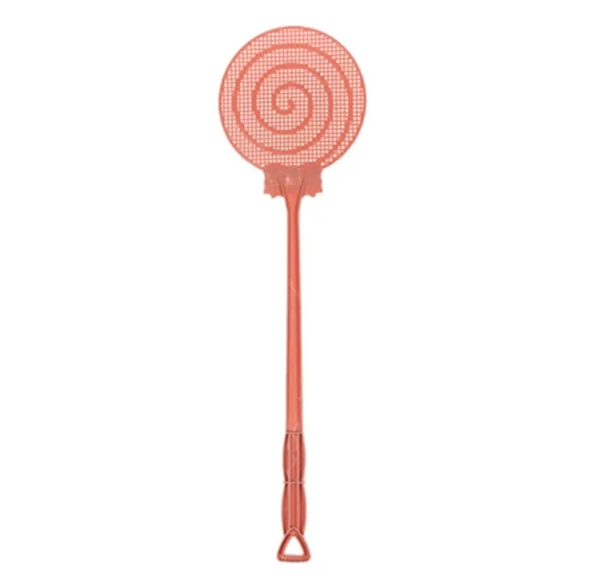
\includegraphics[width= 0.85\linewidth]{vr}
	%		%		\caption{\small\textit{\color{}}}
	%		\vspace*{-10pt}
	%	\end{figure}
%	\textit{Solution.}
%	If no $2$ flies are further than $20$ cm from each other,
%	Minh can strike them all in $1$ strike by aiming the center of the swatter at any fly. 
%	But this is not the case, so let's assume there are $2$ flies, $A$ and $B$, that are more than $20$ cm apart.
%	Then, every other fly is either in a $20$ cm radius of $A$ or in a $20$ cm radius of $B.$
%	Out of the $23$ remaining flies either at least $12$ will be in the $20$ cm radius of $A$
%	or $12$ will be in the $20$ cm radius of $B$.
%	Swatting that the $A$ or $B$ fly with the center of the swatter kills at least $13$.
%	\vskip 0.1cm
%	Thus, by $2$ strikes, he can swat them all.
%	\begin{center}
	%		\textbf{\color{toancuabi}\color{toancuabi}\color{toancuabi}\color{toancuabi}Vocabulary}
	%	\end{center}
%	{\color{toancuabi}Angle}: (dt) góc.
%	\vskip 0.1cm
%	{\color{toancuabi}Application}: (dt)  áp dụng, ứng dụng.
%	\vskip 0.1cm
%	{\color{toancuabi}Contradiction}: (dt) mâu thuẫn, {\color{toancuabi}proof by contradiction}: chứng minh bằng phản chứng.
%	\vskip 0.1cm
%	{\color{toancuabi}Even}: (tt) chẵn, {\color{toancuabi}even number}: số chẵn.
%	\vskip 0.1cm
%	{\color{toancuabi}Knight}: (dt) hiệp sỹ.
%	\vskip 0.1cm
%	{\color{toancuabi}Neighbour}: (dt) người bên cạnh. 
%	\vskip 0.1cm
%	{\color{toancuabi}Midpoint}: (dt) trung điểm.
%	\vskip 0.1cm
%	{\color{toancuabi}Discuss}: (đt) thảo luận, trao đổi.
%	\vskip 0.1cm
%	{\color{toancuabi}Distance}: (dt) khoảng cách.
%	\vskip 0.1cm
%	{\color{toancuabi}Fly}: (dt) côn trùng.
%	\vskip 0.1cm
%	{\color{toancuabi}Finite}: (tt) hữu hạn.
%	\vskip 0.1cm
%	{\color{toancuabi}Hoop}: (dt) vành, đầu vỉ ruồi.
%	\vskip 0.1cm
%	{\color{toancuabi}Infinite}: (tt) vô hạn, vô cùng, infinity (dt). 
%	\vskip 0.1cm
%	{\color{toancuabi}Maximal}: (tt) lớn nhất.
%	\vskip 0.1cm
%	{\color{toancuabi}Minimal}: (tt) nhỏ nhất.
%	\vskip 0.1cm
%	{\color{toancuabi}Olive}: (dt) quả ô-liu. 
%	\vskip 0.1cm
%	{\color{toancuabi}Plane}: (dt) mặt phẳng.
%	\vskip 0.1cm
%	{\color{toancuabi}Point}: (dt) điểm.
%	\vskip 0.1cm
%	{\color{toancuabi}Principle}: (dt) nguyên lý,  {\color{toancuabi}extremal principle}: nguyên lý cực hạn.
%	\vskip 0.1cm
%	{\color{toancuabi}Swatter}: vỉ, {\color{toancuabi}fly swatter}: vỉ ruồi.
%	\vskip 0.1cm
%	{\color{toancuabi}Set}: (dt) tập hợp.
%	\vskip 0.1cm
%	{\color{toancuabi}Strike}: (đt) đập, đánh.
%	\vskip 0.1cm
%	{\color{toancuabi}Table}: (dt) cái bàn, {\color{toancuabi}round table}: bàn tròn, {\color{toancuabi}outdoor table}: bàn ngoài trời.
%	\vskip 0.1cm
%	{\color{toancuabi}Value}: (dt) giá trị.
%	
%\end{multicols}
